\documentclass[onecolumn, draftclsnofoot,10pt, compsoc]{IEEEtran}
\usepackage[utf8]{inputenc}
\usepackage[table,xcdraw]{xcolor}
\usepackage{graphicx}
\usepackage{tabularx}
\usepackage{fancyvrb}
\usepackage{hyperref}
\usepackage{csquotes}
\usepackage{titlesec}
\usepackage{pdfpages}

\titleclass{\subsubsubsection}{straight}[\subsection]

\newcounter{subsubsubsection}[subsubsection]
\renewcommand\thesubsubsubsection{\thesubsubsection.\arabic{subsubsubsection}}
\renewcommand\theparagraph{\thesubsubsubsection.\arabic{paragraph}} % optional; useful if paragraphs are to be numbered

\titleformat{\subsubsubsection}
  {\normalfont\normalsize\bfseries}{\thesubsubsubsection}{1em}{}
\titlespacing*{\subsubsubsection}
{0pt}{3.25ex plus 1ex minus .2ex}{1.5ex plus .2ex}

\makeatletter
\renewcommand\paragraph{\@startsection{paragraph}{5}{\z@}%
  {3.25ex \@plus1ex \@minus.2ex}%
  {-1em}%
  {\normalfont\normalsize\bfseries}}
\renewcommand\subparagraph{\@startsection{subparagraph}{6}{\parindent}%
  {3.25ex \@plus1ex \@minus .2ex}%
  {-1em}%
  {\normalfont\normalsize\bfseries}}
\def\toclevel@subsubsubsection{4}
\def\toclevel@paragraph{5}
\def\toclevel@paragraph{6}
\def\l@subsubsubsection{\@dottedtocline{4}{7em}{4em}}
\def\l@paragraph{\@dottedtocline{5}{10em}{5em}}
\def\l@subparagraph{\@dottedtocline{6}{14em}{6em}}
\makeatother

\setcounter{secnumdepth}{4}
\setcounter{tocdepth}{4}

\newenvironment{changemargin}[2]{%
\begin{list}{}{%
\setlength{\topsep}{0pt}%
\setlength{\leftmargin}{#1}%
\setlength{\rightmargin}{#2}%
\setlength{\listparindent}{\parindent}%
\setlength{\itemindent}{\parindent}%
\setlength{\parsep}{\parskip}%
}%
\item[]}{\end{list}}

% A one to two page document stating user stories
% Requirement example: a user must be able to learn how to use the web press from a remote location
% Don't really need any reference to VR here; that is more of a design choice than a requirement
% Concise; just whatever are the literal requirements that our project must fulfill
\title{Capstone Hand Off Document}
\author{Stephen Hoffmann, Stewart Rodger, Nicholas Pugliese, Kyle Tyler, Symon Ramos}
\date{October 2018 - June 2019}
\newpage

\begin{document}
\setlength\parindent{0pt}
\maketitle

\section*{Overview}
This document describes the design and implementation of the 2018-2019 Senior Design Capstone team 73's project to develop a standalone Virtual Reality training scenario to train someone on an existing procedure for HP's Web Press printers. Our end goal was to develop a prototype that advocates Virtual Reality training as a viable means for HP to pursue at a larger scale.

%TODO TODO TODO: 
%Please make a new file to the right containing all of your weekly reports.
%I already have everyone's tech reviews

\tableofcontents

\newpage

%done, make revisions to team member roles as needed
\section{Introduction to Project}

%    Why was it requested?
%    What is its importance?
\subsection{Project Importance}
This project was requested as the result of a need for personnel and HP customers to be trained on HP's Web Press printers. The current methodology of training requires extensive resources in order to fly customers to a location with an HP Web Press, provide food and a hotel rooms for the duration of the training, and halt any production on the Web Press while the training exercises are running. The current training method also can't account for cases where the Web Press breaks because it's not applicable to break a Web Press for the sole purpose of teaching personnel how to react in that scenario.
\\\\
This project is important to the future of HP as Virtual Reality can prove to be provide a great deal of benefit in regards to the current training procedure of the Web Press printers. While our project served as a means of a prototype, our meetings with HP personnel to discuss and advocate the potential future of Virtual Reality in their training methodology was very successful, leading to much speculation over the potential our project has to assist in the greater vision of the company as a whole. 

%    Who requested it?
%    Who was/were your client(s)?
%    What was the role of the client(s)? (I.e., did they supervise only, or did they participate in doing development)
\subsection{Client Introduction}
Our client and requester for this project was Tim Holt, an employee and representative of HP. Tim comes from a gaming background and has been pursuing a prototype to present to upper management to promote allocation of resources towards the adoption of Virtual Reality training methods for the company's HP Web Press printers. This led to his requesting of a capstone team to further implement such a prototype. Tim fulfilled a role of supervision over our project's direction, providing us with the vision of which to implement our project towards while at the same time approving of the requirements we set for ourselves. We met with him various times throughout this project to discuss the current state of the project and any areas of improvement we could focus on. In large part, most of the developmental procedure was given to our discretion, allowing us the freedom to explore and expand our scenario in what we thought could work best to our advantage. 

%    Who are the members of your team?
%    What were their roles?
\subsection{Team Introduction}
Our team comprised of five members, which, while is more than the average senior design capstone team, worked to our advantage as we were able to clearly define roles in such a way where different aspects of project design and implementation were divided effectively to promote efficient development. We all came from different backgrounds and levels of expertise, greatly enabling our ability to hone in on specific parts of the project. As a result, greater quality and attention to detail was achieved. However, we were nevertheless able to assist each other through paired programming and in such a way that the responsibility of one particular facet was never solely on the shoulders of a particular member for the entire duration of the project.

\subsubsection{Stephen Hoffmann}
Stephen Hoffmann was tasked with the creating the 3D Model of the HP Web Press printer in addition to many various components, such as ink barrels, wipers, and more. With only pictures taken of the Web Press, he was able to implement low-poly but highly efficient and effective representations of the objects to the degree of detail needed to get the point across. In addition, Stephen also implemented many of the interfaces of interactions with various objects, from the opening of the printhead shield to the picking up of objects for additional interaction. 

\subsubsection{Stewart Rodger}
In this project, Stewart Rodger took on the chief role of developing the user interface (UI) for the entire training scenario in addition to the menu. Through the blueprint feature of Unreal, Stewart displayed sound computational understanding by implementing complex and sequential logic to create a workflow that adhered to the standards and design developed in earlier stages. 

\subsubsection{Nicholas Pugliese}
Nicholas Pugliese served as the team's manager and facilitated the overall growth and direction of our project, a role that greatly benefited every team member to a praiseworthy extent. From developing sections of the environment such as the training scenario to becoming, in large part, the focal point of contact between our client and other HP personnel, Nick offered his expertise and support at virtually every aspect of the project.

\subsubsection{Kyle Tyler}
While most of Kyle Tyler's work comprised of the from-scratch development of the environment, the warehouse, and the custom models in the warehouse, Kyle also displayed great versatility in his ability to assist in various aspects of the project, such as his outstanding work with the lighting and textures of the environment, the player rotation controls, and button logic via blueprints. 

\subsubsection{Symon Ramos}
Symon Ramos' contributions in large part encompassed the comprehensive and extensive research of the Web Press printer operator manuals and training procedures as a means to develop and design an accurate and effective training procedure that can easily be translated into Virtual Reality. Symon also implemented various models in the environment, controller scheme designs, and the accompanying audio of the training scenario.


\newpage
\section{Requirements Document}

\subsection*{Revisions}

\begin{table}[ht!]
\begin{tabularx}{\textwidth}{|l|X|X|}
\hline
\rowcolor[HTML]{C0C0C0} 
Section & Original & New \\ \hline
Specific Requirements &  HP needs a less expensive way to train Web Press customers on its operation and maintenance. These customers must receive training that prepares them for the operation and maintenance of the HP Web Press at the same level of competency as the in-person training seminars at an HP Web Press location. Creating an entire training program to replace the current system is not within the scope of this project. Instead, this project will focus on laying the groundwork for a training program and creating a single training scenario that can be used to show the worth of a virtual reality training program.    & Creating an entire training program to replace the current system is not within the scope of this project. Instead, this project will focus on laying the groundwork for a training program and creating a single training scenario that can be used to show the worth of a virtual reality training program.   \\ \hline
\end{tabularx}
\end{table}

\subsection*{Client Verification}

\begin{Verbatim}[frame=single]
Nick this is good - happy to sign off on it.

-Tim Holt [2019-04-19, 13:22]
\end{Verbatim}

% What are a few things that are fundamental to the program?
% What is the big idea -> user needs to learn web press remotely
\subsection{General Requirements}
There is a need for personnel and HP customers to be trained on HP's Web Press printers. The current methodology of training requires extensive resources in order to fly customers to a location with an HP Web Press, provide food and a hotel rooms for the duration of the training, and halt any production on the Web Press while the training exercises are running. The current training method also can't account for cases where the Web Press breaks because it's not applicable to break a Web Press for the sole purpose of teaching personnel how to react in that scenario.

% What are some requirements specific to a certain part of the project?
\subsection{Specific Requirements}
HP needs a less expensive way to train Web Press customers on its operation and maintenance. These customers must receive training that prepares them for the operation and maintenance of the HP Web Press at the same level of competency as the in-person training seminars at an HP Web Press location. Creating an entire training program to replace the current system is not within the scope of this project. Instead, this project will focus on laying the groundwork for a training program and creating a single training scenario that can be used to show the worth of a virtual reality training program. 

% Inputs/Outputs -> need computer, some kind of input device, visual output
% \subsection{External interfaces}
The customer must have access to facsimiles or analogs of the HP Web Press technology in order to gain familiarity with the real product. When they use a real Web Press for the first time after the remote training they must feel familiar with the physical hardware.

Customers with no prior industrial printing experience should be able to complete the training with adequate knowledge retention.
% Measurable effectiveness
% Efficiency
% Satisfaction criteria in specific contexts of use
% \subsection{Usability}

% Frame rate
% Number of simultaneous users supported
% Load times
% I think performance (and other non-functional requirements) are a design document item, not solution requirements -N
%\subsection{Performance}

The new training program must also be more preferable by HP than their old training program and cause them to consider adopting this new method instead.

% Constraints on the program imposed by external standards, regulatory requirements, or project limitations
% Ex: OS constraints, memory, etc
\subsection{Constraints}
The training program should be significantly less expensive per customer to complete than the current in person training model. Ideally there should be no transportation or food expenses to account for. The customer should not have to leave their home or place of business to complete the training. It should be accessible to customers anywhere in the world that has an internet connection. The solution should only include existing HP products utilize preexisting business agreements HP possesses with current technology leaders. 

\subsection{Gantt Chart}
\bigskip
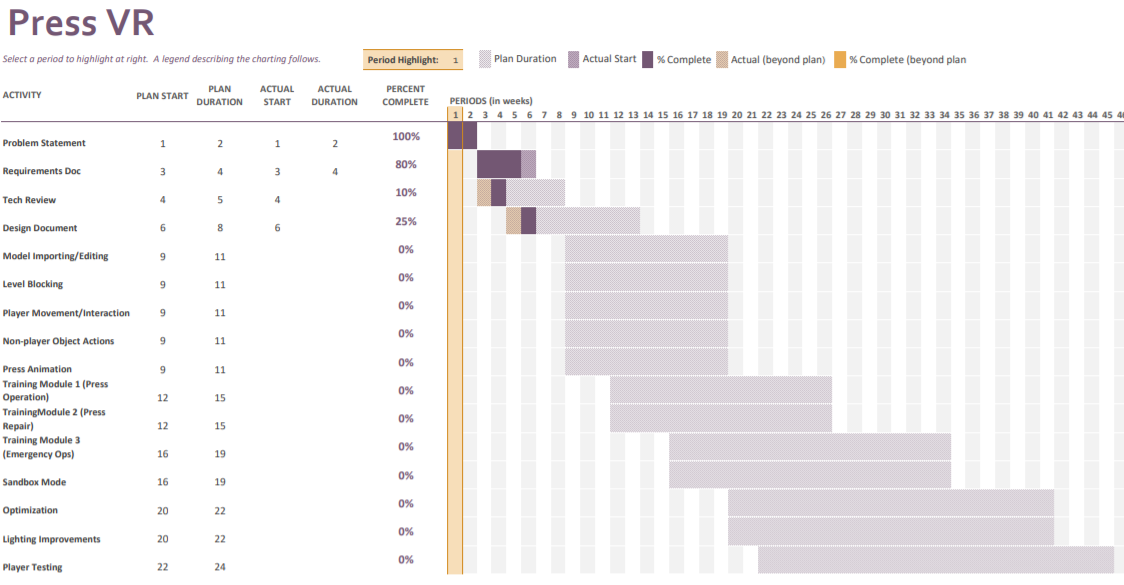
\includegraphics[scale=.75]{ganttChart.PNG}


\newpage
\section{Design Document}
        Proposed is a training program capable of providing the same level of training from a remote location away from real HP printer technology by the use of a virtual reality simulations. The program will contain several different modes and scenarios to be used in place of actual training on the HP facility.
\newpage

\subsection*{Revisions}

\begin{table}[ht!]
\begin{tabularx}{\textwidth}{|l|X|X|}
\hline
\rowcolor[HTML]{C0C0C0} 
Section & Original & New \\ \hline
Scope &     The software to be produced is to be called Web Press VR. This software product will allow users to learn how to use
an HP PageWide Web Press in a completely virtual environment. Users will be able to use a Web Press virtually in a
sandbox mode, a full training mode, and specific skill training modules. Letting users explore a Web Press in a sand
box mode will give the user familiarity with the Web Press that will carry over into the real world. A full training mode
will allow users to see what it is like to use a Web Press, from the beginning to the end of an operation cycle. The skill
training modules will allow users to familiarize themselves with specific tasks and operations one may wish to perform
with a Web Press.     &   The software to be produced is to be called Web Press VR. This software product will allow users to learn how to use
an HP PageWide Web Press in a completely virtual environment. Users will be able to use a Web Press virtually in a
sandbox mode, a full training mode, and specific skill training modules. Letting users explore a Web Press in a sand
box mode will give the user familiarity with the Web Press that will carry over into the real world. A full training mode
will allow users to see what it is like to use a Web Press, from the beginning to the end of an operation cycle. The skill
training modules will allow users to familiarize themselves with specific tasks and operations one may wish to perform
with a Web Press. Our goal is to facilitate the creation of a program, and to construct a prototype that can be shown off as a feasibility test to management at HP. This prototype will serve to create the conversation that money should be spent internally at HP to develop the VR program further.  \\ \hline
\end{tabularx}
\end{table}

\subsection*{Client Verification}

\begin{Verbatim}[frame=single]
Nick this is good - happy to sign off on it.

-Tim Holt [2019-04-19, 13:22]
\end{Verbatim}

\clearpage



% 8. now you write!

\subsection{Overview}
\subsubsection{Scope}
The software to be produced is to be called Web Press VR. This software product will allow users to learn how to use an HP PageWide Web Press in a completely virtual environment. Users will be able to use a Web Press virtually in a sandbox mode, a full training mode, and specific skill training modules. Letting users explore a Web Press in a sand box mode will give the user familiarity with the Web Press that will carry over into the real world. A full training mode will allow users to see what it is like to use a Web Press, from the beginning to the end of an operation cycle. The skill training modules will allow users to familiarize themselves with specific tasks and operations one may wish to perform with a Web Press.

The benefits of using virtual reality to train people to use the Web Press are reductions in training costs, reductions in time required to train, and increases in total understanding of the system. An ultimate goal of the system is to streamline to whole training process, and to serve as a viable alternative to in-person training. We aim to show that virtual reality is an invaluable training tool, and has uses beyond just the scope of this particular product. Our goal is to facilitate the creation of a program, and to construct a prototype that can be shown off as a feasibility test to management at HP. This prototype will serve to create the conversation that money should be spent internally at HP to develop the VR program further.
\subsubsection{Purpose}
The purpose of our software is to be a virtual reality training application to work with modern virtual reality headsets. By taking advantage of the increased accessibility of virtual reality as well as the decreased cost of hardware, we hope to build an application that will reduce the costs associated with training people to use HP's PageWide Web Press product line. Developing these training scenarios will improve the effectiveness of HP's current training procedure as well as mitigate the costs and risks of handling real machinery by the trainees.
\subsubsection{Intended Audience}
The intended audience of our software will ultimately be personnel who are enrolled to be trained on HP's PageWide Web Press product line, whether it be HP employees or customers who have purchased the technology. Teachers and supervisors of the training program of HP would also be involved in the utilization of our software. Relative to the scope of our project, we intend for our software to be reviewed in-depth by our client and any other potential personnel that our client recommends. Our client will use our software as an additional means to prompt upper management of HP to invest and allocate more resources into the development of VR software that trains personnel on PageWide Web Press use. 
\subsubsection{Conformance}
The ultimate goal of the VR system is to provide an environment that allows the user to receive the same quality of training as if they were participating in an in-person training event at an actual HP PageWide Web Press location.

\subsection{Definitions}
\begin{enumerate}
    \item Virtual Reality (VR) - A simulated computer environment that immerses the user in a 3D space
    \item PageWide Web Press - Industrial HP printers for commercial printing. "PageWide" refers to the length of the printhead matching a standard 8.5"x11" piece of paper. Web refers to the name of the roll of paper to be printed
    \item Headset - The VR component worn on a users head to providing visual and audio immersion
    \item CAD - Computer Aided Design. Also the file type used for 3D models that represent real life objects, usually to exact specifications
    \item GitHub - A website git tool used for version control when building software
    \item Frame rate - The frequency at which a graphics program outputs frames of video.
    \item Refresh rate - The frequency at which a display updates its image. Usually measured in refreshes per second (Hz)
    \item GPU - The graphics processing unit, the device in charge of rendering and outputting on to display
    \item HDMI - The display cable used to connect a VR Headset to a computer
    \item Blueprints - Blueprints Visual Scripting. A node-based interface for creating gameplay elements in Unreal Engine
    \item Object Oriented (OO) - A programming methodology that enables a system to be modeled as a set of object that can be controlled and manipulated in a modular manner
    
\end{enumerate}
\subsection{Conceptual model for software design descriptions}
The proposed system will provide the training in the form of a virtual reality re-creation of the HP PageWide Web Press using the Unreal Engine as a graphics solution. HP will provide 3D CAD models of the Web Press to be use as a baseline for developing our own interactive models. The models in the final application must be recognizable as real Web Press products to ensure high correlation between the knowledge received in the training program and the situations involved with running a real web press.

The core of the program will be a set of training exercises that prepare different scenarios for the user such as fixing a broken part or restocking the machine with paper. The user must complete these objectives before they will receive a certification for that particular exercise.
\subsubsection{Software design in context}
The product will consist of one bundled application. The application will manage all aspects of the program, from booting, saving, and exiting. It will be required to have a headset running and connected to the computer to functionally run. A save folder will be kept for user preferences and performance metrics, and the application will only use system resources when a user is actively engaged with the headset on. No databases, networking, or external resources will be required to run the application. Everything will be handled inside the program bundle.

% Hardware interfaces
Required hardware for the software product include a virtual reality headset, a pair of virtual reality controllers, a computer with HDMI and USB support, and a discrete graphics card. The target virtual reality headset is the HP Microsoft Mixed Reality Headset, but the software should be designed to support the Oculus Rift, the Vive, and most other consumer VR headsets. The software will also require the use of a pair of virtual reality controllers, and those controllers must be compatible with whatever headset the software user chooses to use. The HP Microsoft Mixed Reality Headset requires one USB port and one HDMI port, but other headsets may require more input options. This headset also runs on relatively low end graphics cards, but other headsets may require a more powerful GPU. 

% Software interfaces
The only required software product needed to run the application we are developing is the Windows 10 operating system. Developing for other operating systems is out of the scope of the project at this time. 

% Memory constraints
There are no hard memory constraints on the software product, but the an application with a smaller memory footprint will allow the application to be more quickly installed and more easily run on systems with limited memory space. 
\subsubsection{Software design descriptions within the life cycle}
\begin{center}
    \begin{figure}[h]
        \centering
        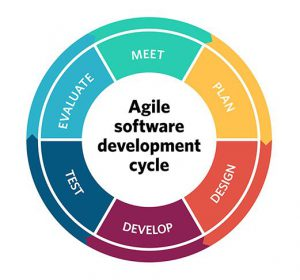
\includegraphics[width=10cm, height=9cm]{agile.jpg}
        \caption{The Agile Development Cycle. Adapted from \cite{1}.}
        \label{fig:mesh1}
    \end{figure}
\end{center}

We will be implementing an Agile development cycle for our project, as displayed above in  figure \ref{fig:mesh1}. This methodology emphasizes an active and collaborative approach to the software development life cycle. It involves designing, creating, and testing multiple iterations of the program and constantly evaluating its state with our client. Certain aspects of Agile development include gradual modifications to requirements, incremental versions of the program, frequent deliveries on products, integrated testing, and constant collaboration with stakeholders \cite{1}. We chose this development cycle to preemptively prepare for possible situations where we find that one design works better than another. The ability to change our direction to what would produce the best, most viable training module is a tremendous benefit that could assist in the probability of our success. While some aspects of the Waterfall methodology (which emphasizes a sequential progress flow) should be considered, such as adhering to overarching requirements and the general design format that our client would like to see in addition to comprehensive documentation, having the flexibility of Agile development will allow us to build a product that the client will more likely approve of.  

\subsection{Design description information content}
\subsubsection{Introduction}
This section will contain the following: an identification of the software design descriptions, identified design stakeholders, identified design concerns, selected design viewpoints, design views, design overlays, and design rationale.

\subsubsection{SDD identification}
In order to substantiate and validate our progress, the performance metrics established in our Problem Statement document will be addressed. The performance metrics specify certain aspects of our project that we will strive to complete. At several points in our project's duration, we will measure our progress based on the metrics below:

\begin{enumerate}
\item A VR environment is constructed with a PageWide Web Press in the scene. This environment should include recognizable graphics, sounds, and appear to represent a real world work environment to a reasonable extent.

\item The user can move around within the scene using the provided VR headset, and the user can interact with the press in at least one way using the provided controllers. 

\item The interactive parts of the VR press simulate at least one major function in virtual reality that would be covered in the physical reality training. Instructions should be given to the user with in-game audio and visual cues.  

\item The virtual reality press simulates failure when the VR press is operated incorrectly (controls used in the wrong order) in at least one (ideally all) of the functions in the training.

\item Outside individuals with no prior knowledge can complete the training successfully, without triggering a failure (when allowed repeat attempts), using only the instructions and prompts within the VR simulation. 

\item Positive user feedback on interaction and intuitive gameplay mechanisms, especially for users with no background in virtual reality or gaming controls in general.

\item Framework that can be used to easily implement future training scenarios after completion of capstone.

\item After completing the VR training program, users can correctly identify parts and functions of the real press that were covered in the program.
\end{enumerate}

The basis of our verification will be predicated on HP's evaluation of our performance. The performance metrics will prove to be useful as specific goals to strive for, but ultimately, HP and our client will determine the validity of our project. 

\subsubsection{Design stakeholders and their concerns}
Because of the fluid circumstances of our project, our client, Tim Holt, has defined our project goal to be that of a self-encapsulated program that contains a basic training module. An important aspect to our relationship with our stakeholder would be consistent interaction through weekly meetings in order to ensure that we are on the right track. Because of the limited time we have to develop the program, it is imperative that we actively ask questions and review our progress with our client on a regular basis. 
\subsubsection{Design views}
The main assumption in this document is that the contents of the training exercises/scenarios will be determined by HP during design planning meetings with Tim Holt, the project sponsor as development starts. We have not yet received technical manuals or descriptions of existing training seminars and as such have not been able to go through the these materials to gain an understanding of the contents of the scenarios.
\subsubsection{Design viewpoints}
At the conclusion of our project, we will have created training modules capable of being used with a correctly configured, mid-tier laptop and an HP Mixed Reality Headset. Resources include the CAD files and programs used to implement the modules. The program must be capable of being shared across physical distances so personnel can use it remotely. The documentation and instructions must also be clear and concise. For verification purposes, the personnel running the training modules can provide feedback in addition to any leadership supervising the training for the Web Press systems. One contingency to note is the demand for these training modules; if we had a limited number of personnel to train for the first time, we might not be able to receive enough feedback to properly make a case for the advancement of VR training for HP Web Press systems. 
\newpage

\subsubsection{Design elements}
% Design Entities
The following is a list of design entities with a description of their attributes, which include name, type, and purpose:

\begin{itemize}
    \item Name: Unreal Engine\\
          Type: Framework / Engine\\
          Description: A 3D engine from which we will build our application 
    \item Name: Blueprints\\
          Type: Generic templates\\
          Description: A set of functions in Unreal Engine to be used for visual scripting to reduce programming time
    \item Name: Sandbox Mode\\
          Type: Module\\
          Description: A portion of the program designed to allow users to freely interact with the 3D environment in an undirected setting 
    \item Name: Training Mode\\
          Type: Module\\
          Description: A portion of the program designed to allow users to be given a set of instructions that they must follow to complete some task
    \item Name: Player Controller\\
          Type: Component\\
          Description: A component which will allow the user to interact with the 3D environment, receiving input from a virtual reality headset and pair of controllers
\end{itemize}

\subsubsection{Design overlays}
% Business Analysis
Although we will have definitive methods with which to analyze the development of our modules, we will also begin the verification process during the business analysis portion of our project as well. Our design will require an extensive amount of verification as well in order to create as optimal and accurate a module as we can. Within our business analysis, we will be gathering data from previous virtual reality studies, instruction manuals, current training programs, and other resources to assist in the design of our modules. We will need to verify our design in terms of our use cases during every step of development. We will also speak with personnel involved with training in order to support our design plan for each module that we will strive to create. 

% Code/Documentation Sharing and Accountability
The management of our documentation, assignment submissions, code, CAD models, audio and video, notes, photos, and version control repositories will be a major factor that could allow us to provide a quantifiable measure with the resources we are developing. Software we will use will be Google Drive, Overleaf, and Github to share our code and documents. Verification will also involve monitoring the progress of each of our team members. By keeping each other accountable in the development of our tangible progress, we can strive for the optimization of a better product. 

% Talking with client
Among our requirements will be to regularly hold meetings with our client and be in constant discussion about our progress. We will be holding weekly meetings either at HP or on campus with our group and our client where we will go over our recent development and state our goals for the week. We will also document our progress on our individual class blog as well as within an informal work log. Emails will also be used to coordinate between our client throughout the week. In terms of our group dynamic, we will be communicating most often using Slack. In addition, we will also hold weekly meetings with our TA, Christopher Kawell for the class, updating him on our progress both as a group and individually. These meetings will be held in a scrum format where we will discuss what we've done and what we are planning to do. 
\subsubsection{Design rationale}
Many components of our project, such as which VR headset to use, have been predetermined by our client and is only subject to change should we have a justifiable alternative that could prove to be more beneficial to HP. As such, we will be using the Mixed Reality Headsets manufactured by HP as our hardware. Software-wise, we are going to use the Unreal Engine as it contains many design components that we would like to use in order to create our modules. 

The management of our code and documentation will be done using the software described in the "Design overlays" section (Google Drive, Overleaf, and Github) due to each software's ease of access and applicability for each task. 

The metrics used in the "SDD identification" section were included as a means to outline the items we should strive to accomplish. While some of the items are general, some are specific so as to emphasize the importance in crafting a detailed simulation that can improve user experience. This will aid in HP's evaluation of our performance. 


\subsubsection{Design languages}
The design language we are choosing to take advantage of is one that is a feature of Unreal Engine, which is Blueprints Visual Scripting. This design language is a system in Unreal Engine that acts as a complete gameplay scripting system that is based on the concept of using a node-based interface to create gameplay elements in the Unreal Editor. It is used to define object-oriented classes or objects. The system will allow our designers to implement features that would normally require writing code, and so will cut back on total development time. Any features that do not have a Blueprint solution will be implemented via programming, but most of the basic functionality of our system will be created using this system.

\newpage

\subsection{Design viewpoints}
\subsubsection{Introduction}
This section will describe several design viewpoints. It will illustrate these viewpoints in terms of design language selections, relates design concerns with viewpoints, and establishes language neutral names for these viewpoints. 

\subsubsection{Context viewpoint}
The environmental conditions will cover room-space requirements and safety measures for user and equipment.

The training application will be designed for room-scale VR with 3x3 meter available space in mind. Less space would still function well, but will allow for less physical user motion, such as stepping forward, leaning, turning, and stretching arms. 

The following simple protocols to setup the room environment will ensure safety of equipment and the user:
\begin{enumerate}
    \item Clean surrounding areas of all objects
    \item Ensure cables are not twisted
    \item Use the controller wrist straps
    \item Understand user's physical boundaries
\end{enumerate}
\subsubsection{Composition viewpoint}
The user will interface with the training program through a virtual reality headset. There are 2 main types of virtual reality headsets; built in motion camera headsets and external camera headsets. While the primary headset for the program will be a built in motion camera headset, Microsoft Mixed Reality, the training program will be equally compatible for both types of headsets.

External camera headsets use 1 or more cameras placed away from the headset. The field of view created by the camera(s) is the area that the headset and controllers can be moved within. With a built in motion camera headset, there is only 1 camera, built into the headset itself, and its forward facing field of view is the area the controllers can be moved within. Both have their own flaws. With the former, the headset can not move outside the play area, leaving the in game avatar stuck in place. With the latter, the controllers must be in front of the user, if the user tried to place their controllers above their head or behind them the controllers would become stuck at the edge of the viewport. 

The training program will use standard interface mechanics and inputs to guarantee cross compatibility with other forms of virtual reality headsets. Specifically, the program will highlight objects that can be interacted with, and will present button prompts to show which button is used to interact with the object.  

The VR application will be built for windows 10 systems, knowing that the primary headset will be HP's Windows Mixed Reality headset. No other third party software will be needed. This includes distribution software such as Steam.
\subsubsection{Logical viewpoint}

The training program will be structured as a series of menus presented to the user. These menus will control which of the training modes and scenarios are presented to the user for completion. Figure \ref{fig:logic_uml} describes the flow of logic through the menus and selecting the training mode, with stop conditions for each state. The training program will be structured in the form of a modern video game. Users will be given scenarios to perform and must complete the requirements of said scenario in order to pass and receive qualification. These qualifications will be stored on a per-user basis to prove to the proctor that the user has indeed passed the training.

\begin{center}
    \begin{figure}[h]
        \centering
        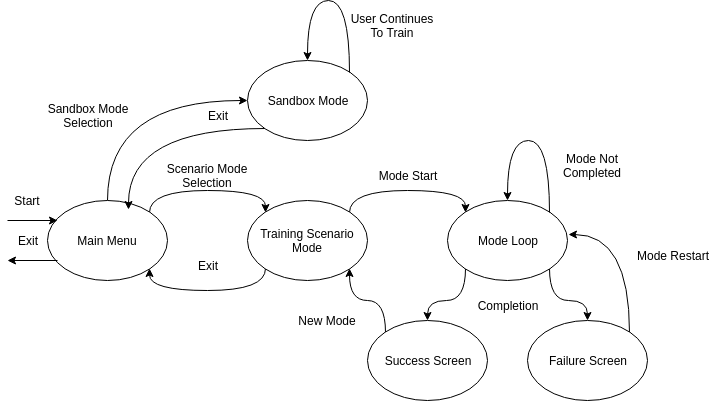
\includegraphics[width=15cm, height=9cm]{logical_view1.png}
        \caption{UML Diagram for the logic flow of the training program.}
        \label{fig:logic_uml}
    \end{figure}
\end{center}

\subsubsection{Dependency viewpoint}
The training program must contain a 3D recreation of the real HP Web Press in order to provide the most accurate training possible to the user. As much as possible, the program must behave in the same way as a real Web Press. HP will provide high quality 3D computer aided design files that can be imported into the Unreal Engine for our use.

Unfortunately, these CAD file might prove to be too detailed for our programs use. The goal is to have a training program that can be run on a middle tier priced laptop, and if the CAD files are too large in file size and detail it will cause the laptop to not be able to run the program at the desired frame rate.

In this event, we will redesign the CAD files to a more simple design to allow for the program to run at a smooth and stable frame rate.
\subsubsection{Information viewpoint}
There are only a few cases in which information is being managed for the user:
\begin{enumerate}
    \item Saving user scores
    \item Saving users records of completed training
    \item Saving user preferences
\end{enumerate}
All data will be stored locally on the machine the game is played on. No data is sent to or retrieved from the internet after the application has been installed. 

% Data Gathering and Analysis
After we develop our modules to the extent where we can begin user testing, we will want to quantify our project's performance by gathering data to analyze. As the purpose of our modules will be to train individuals on how to operate Web Press technology and based on our defined performance metrics, we will utilize the following to analyze our effectiveness: 
\begin{enumerate}
    \item User Feedback
    \item Efficiency in performing certain tasks
    \item Ability to implement new training scenarios
\end{enumerate}
Testing the system interface will be fully dependant on user feedback. We can develop objectives for the user to complete, such as mundane tasks like picking up objects and dropping them, to more complex scenarios. Feedback on interfaces will be based on a criteria of topics with questions pertaining to each. Questions will include asking how intuitive the task feels with little to no instructions, how responsive actions are, tester likes and dislikes about the functionality of in-game actions, and suggestions on what testers think they could benefit from.

Testing will involve the creating an user-name and completing training, while closing the game between each completion to ensure the data is been saved and loaded properly. To test the saving of user preferences the preference will need to be changed and the game will need to be reset to verify changes.

\subsubsection{Policies and regulations}
Policy will be dictated by HP. This system will belong to them as a HP licensed product. We as a development team will own no rights.

Official HP resources will be made available to this team under a non-disclosure agreement. These reference materials are not to be used in the final product, and instead are to be used in the creation of derivative models and works that will not fall under the non-disclosure agreement. The final program will be freely available to be shown off at the OSU Engineering Expo as part of the senior project capstone class.

\subsubsection{Interface viewpoint}
% User interfaces
The user interfaces of the software product necessary to accomplish the software requirements include a virtual reality display of 3D environments, a navigation interface for users to move through a 3D space, and text UI elements to allow a user to access information in the application. It is important that the software product is comfortable and understandable for users. Virtual reality can adversely effect users who are sensitive to motion sickness, so a consistent frame rate in the application is important for user comfort. Users must also be able to understand their environment and clearly see what options are available to them, such as where they are able to move and what they are able to interact with.

\subsubsection{Interaction viewpoint}
The training program should be accessible to everyone. No prior virtual reality or video gaming experience should be necessary to complete the training exercises provided by the program.

One of the biggest steps taken to keep the training program approachable will be the availability of different movement options for the user. The most common movement style in a typical VR game is teleportation: the user holds on button down on the controller and an indicator appears pointing to the location the user will be teleported to if they press another button. The user may move the pointer to a new location by moving the controller around in the virtual space, or they may cancel the movement command with a button press. Of course, the user will be able to physically walk around the real world and observe the same movement in the virtual world, but teleportation allows the user to have free reign of movement throughout the entire virtual space and not be limited to the dimensions of the physical surroundings.

Additionally, the user will be able to move around with the traditional gaming style of pointing the analog stick in the direction they want to move. This option will have to be opted into by users as the consensus of virtual reality players is that movement in this manner tricks their eyes into believing that there is actually physical motion occurring without movement from the legs, which has a high percent chance to cause nausea.

%Move this? ---> is this true?
% this should still be true. -nick
After the user completes a scenario or section of scenarios they must take a quiz about what they just accomplished. If they do not meet an information retention rate of at least 90\% they must complete the scenario or section of scenarios again until they are ale to achieve 90\% retention or better.

Additionally, some scenarios may be time dependant and require the user to finish the scenario requirements in the allotted time. If they do not complete the scenarios in the allotted time the scenario is marked as failed and the user must attempt that scenario again before they are allowed to take that scenario or scenario section quiz and move on to different scenarios.
\subsubsection{State dynamics viewpoint}
The training program will have two modes: scenario and sandbox.

Scenario mode puts the user into a predetermined event or series of events and requires them to participate until the desired outcome is achieved, or other limitations like a time limit runs out. For instance, one such scenario would be if the Web Press breaks down or has stopped printing the user must investigate the problem and return the press to a nominally functioning state. A subsection of the scenario mode will be the alarm gauntlet: a series of scenarios designed to test the users knowledge of the Web Presses many alarm systems and how to silence them by fixing the associated fault.

Sandbox mode is more free form. There is no time limit or overarching goal to achieve. Sandbox mode allows the user to interact with the Web Press as if they were standing next to a real one in person. The user may practice any feature of the Web Press they desire and the Web Press will respond as expected. Sandbox mode allows for user to test things they might not get to test on the real Web Press such as what happens if the Web Press's paper feeder jams and is not fixed in the proper amount of time, and what happens to the rest of the system as a consequence.

The significance of having both modes available allows personnel to first be trained to be trainable (via the sandbox mode) by familiarizing themselves with both Web Press and VR concepts. This invites them to succeed. Scenario mode, however, will teach the user how to deal with specific events, providing them with practical experience and can be more valuable in than sandbox mode in that it prepares the user how to handle such events, such as the Web Press breaking down. To justify and validate the use of two modes, user feedback will be gathered by HP personnel to inquire on the effectiveness of having scenario and sandbox mode.

\subsubsection{Algorithm viewpoint}
The goal will be to have four separate controller classes; Player controller, Quest-State Controller, UI controller, and Object Controller. From a high level viewpoint, each controller will use a modular class based design to allow expansion of features and modifications based on specific level design.

Each controller will be in charge of a different portion of user interaction and feedback, while also working together to provide a full experience.

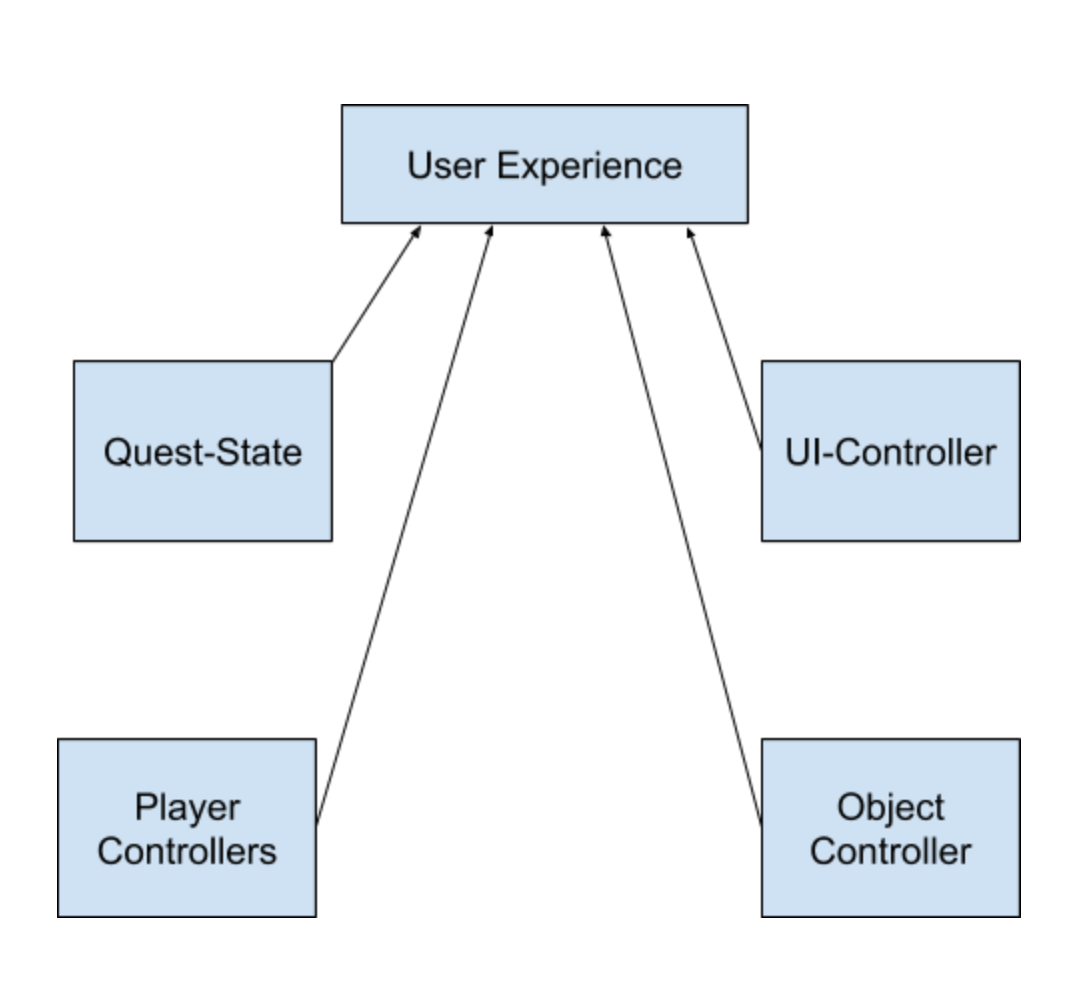
\includegraphics[width=200pt]{AlgoDia.png}

\subsubsubsection{Player Controller}
The Player Controller will be in charge primarily of player input and translating that information into the virtual world. The Player Controller will also be in charge of all variables related to the player, such as player scores.
\subsubsubsection{Quest-State Controller}
The Quest-State Controller is in charge of all task oriented logic and the current state of the quest events.
\subsubsubsection{UI Controller}
The UI Controller will be managing all UI displayed to the user on screen. This includes touchable floating text, buttons, and scores. The variables for these variables will be referenced from the Player and Quest-State Controller.
\subsubsubsection{Object Controller}
The Object Controller class will be what all non player objects inherit, such as interactive objects. This will be in-charge of when an object can be initialized or destroyed, and whether or not it contains physical properties or other unique characteristics.

\subsubsection{Resources viewpoint}
Since this program will be run as an Unreal Application on internal company servers and computers, security will not be a major focus. Our team does understand that some printer models will not be of public knowledge (secret), so any public demo will use only public printer models.

As far as data security is concerned, all files will be built and compiled using Unreal for internal use only. We will not be implementing any method to protect assets, such as CAD models, from being stolen from the company's internal servers.
%\subsection{Bibliography}
\begin{thebibliography}{}
\bibitem{1}
Project-Management, “10 Key Principles of Agile Software Development,” Best Project Management Software Reviews, Oct. 8, 2018. [Online]. Available: https://project-management.com/10-key-principles-of-agile-software-development/ [Accessed: Nov. 27, 2018].
\end{thebibliography}


\newpage
\section{Tech Reviews}

\subsection{Nicholas Pugliese}
\subsubsection{Introduction}
Our project is to create a virtual reality simulation in order to teach the user how to operate and maintain the HP Web Press from a remote location, augmenting the existing in-person seminars that HP holds for customers. The training program will share many of the same characteristics as a video game, and our team will utilize video game design principles to teach the user how to use the Web Press. This shift in paradigm changes how information will be passed to the user and how the user will be tested for knowledge retention. This tech review will compare and contrast "classroom" environments such as a traditional lecture/seminar style of teaching versus that of an interactive video game/program. The "technologies" being reviewed are methods of education, which can be classified as technology based on the first definition of technology from Merriam-Webster.

\begin{displayquote}
"\textbf{technology}: the practical application of knowledge especially in a particular area"
\end{displayquote}

\subsubsection{Traditional}
The most common style of in-person teaching is the lecture format. Lectures involve a speaker or speakers talking to a large number of students about a topic or topics. While lecture formats are usually enhanced by means of visual aid in the form of either physical objects or a slideshow of images, they are generally oral communication. Students in lectures take notes and memorize lessons to retain information \cite{lecture}. An in-person lecture has time set aside during class for questions and clarifications. Achieving the same student/teacher interaction can be difficult in a remote environment. Prerecorded lectures also exist, and those may serve distance learning students better because they have the ability to pause and go back to rewatch a section over to let the information sink in and take better notes. However, this method lacks the near-instant feedback a student can receive by asking a question directly to the lecturer.

Lecture formats are really good at teaching ideas and concepts. Learning how to operate a machine requires hands-on experience. A format for teaching this kind of hands-on knowledge, is often a laboratory or "Lab" class. Lab classes are usually longer than lectures (usually lasting 2-3 hours) and involve completing a task or tasks and documenting what happened in a formal write up. Lab work is usually a more-involved task that acts like a piece of homework. Another benefit of a lab format is that the lab teacher is present and can be asked questions.

Lecture based formats allow experts to share their knowledge directly with the students. It is a great method for hammering in information in sequence that builds upon itself and can include showing example equations as well as work that can be done in class with pen and paper. This style would lend well to general information about the Web Press. However, the ceiling for useful skill knowledge can only reach so high. If a lecturer is describing how to do an action the student can write it down and memorize it, but there are fundamental lessons (such as learning to operate machinery) that can only be taught through through experience.

\subsubsection{Video Games}
Video games have the ability to implicitly teach the player with actions rather than words. For example, the video game Portal by Valve revolves around the namesake device the "portal gun." The gun is capable of firing two portals, one orange, one blue, on a surface. If you pass through one portal you appear out the other. The tutorial of Portal demonstrates this ability to the player by placing the device on a rotating pedestal in the center of a room. The player is forced to wait inside of an anti-chamber to the room the Portal Gun is in, connected by a locked door and a window. Inside the room the orange portal is stationary on a wall the player can clearly see and as the portal gun revolves it fires the blue portal onto different walls in the room. The player is encouraged to watch what the portal gun is doing simply by having nothing else to do in the room. Because of this funneling of the player's attention and subtle display of the game's main mechanic, the player has learned what they will need to do for the majority of the game without having to resort to a voice over or an essay of text giving instructions. The player has been taught without breaking immersion. \cite{portal}

Half Life 2 by Valve uses this experimental style of teaching to pass knowledge to the player. In the beginning tutorial of Half-Life 2 the player is put into a room with several wooden creates and a wooden barricade placed over the exit door. Placed in the center of the room there is a metal crowbar. Through experimentation the player must realize that they can smash the wooden crates and eventually the obstruction over the exit door. This implementation of the experimental tutorial is different from the one in portal that is more guided. In Half-Life 2 the player may sit in the room for as long as they wish. The game will not prompt them to continue. It is solely player-diver to proceed in the game. This situation presented to the player early in the game sets the tone that things may be played around or experimented with, and that behavior will be rewarded.
\cite{hl2}

\subsubsection{Comparison}
Video games have the ability to create situations like in Half-Life where it is up to the player/student to figure out how to proceed. This engagement requires the student to use their critical thinking skills rather than memorize information from a book or lecture. As the old proverb says" "If you give a person a fish, they will eat for a day. If you teach a person to fish, they'll eat for a lifetime." The essence of this is that learning how to do something lays the foundation of understanding so you can replicated the actions in the future. This is why creating a virtual reality training program will be vastly better than just recording a bunch of videos for the customers to watch. If they customers are engaged in their learning and have to figure things out they will not only retain more knowledge but also be able to apply the lessons learned to different situations in the future.

Nick Babich in an article he wrote for Adobe says:
\begin{displayquote}
"Too much information received in a short period of time can easily overwhelm students. As a result, they become bored, disengaged, and usually not sure why they are learning about a topic in the first place." \cite{adobe}
\end{displayquote}
Granted, there are some students who will thrive in a fact-memorization environment. Part of the recommendation of this paper is to create two modes for our project to account for these different learning patterns from different kinds of people. The main area that can be explored in VR that can't be taught in lecture is this sense of experience. Babich also writes:
\begin{displayquote}
"When students read about something, they often want to experience it. With VR, they aren't limited to word descriptions or book illustrations; they can explore the topic and see how things are put together." \cite{adobe}
\end{displayquote}
With this added tool of visual learning students that might have been struggling to understand a concept can immediately see the merit of what they are being told to do. Results can formulate right in front of their eyes that reinforces their understanding of the material.

Video games can embody this experimentation style of learning because they can create invisible barriers or teaching devices (such as the door unlocking only after you watch the portal gun for a while) that still act as a teacher, but are player reliant. This style of teaching by experimentation won't appeal to all students or players, but for the ones it does it creates a sense of accomplishment and internal motivation that bolsters the student/player's desire to play or learn more.

This style of putting the player in a metaphorical box is one that is not unique to new media such as video games and virtual reality, it has existed in the form of puzzles for a very long time. Teaching via puzzles like the ones in video games uses the same techniques as a laboratory class: forcing the student to solve a problem using a limited set of information. Video games intrinsically have to employ this technique because game (and virtual reality programs) are interactive experiences. Not all games use the Portal and Half-Life 2 style of tutorial. Some games present the user with text descriptions of actions and the user must read to find out what things do. This tactic of bringing the user outside of the game to teach is not considered to be effective. \cite{tutorials}

\subsubsection{Recommendation}
For our project, I recommend to our group that we focus on creating a learning environment for two types of learners: those who learn by reading or from lectures ("readers"), and those who learn by doing ("doers"). This division of learners is made because virtual reality allows for the creation of an almost one-to-one ratio of real life hardware to virtual reality simulation. This simulation provides a large boost to the retained knowledge of "doers" because they are allowed to learn by experimentation and get to see a firsthand account of the knowledge in action. For "doers" a training mode will be created using the style of tutorials from Portal and Half-Life 2. This mode is analogous to a sandbox learning environment where the user has a goal, but no set of rules or guidelines to achieve that goal. They are free to do as they wish as long as the overarching task is completed. Our group will be examining more video games such as Portal and Half-Life 2 to find more example of good tutorials by experimentation to base the sandbox training scenarios off of. To keep the learner on track, a series of checkboxes or progress meters will be displayed on the heads-up-display of the user-interface. These progress meters don't specify how to complete their goals and instead only track if they have been completed. This visual indicator of program will help the "doers" to stay motivated in experimenting with the sandbox.

The second learning environment I recommend our group to make is one for "readers." Learning by fact retention still remains a valid method of teaching, as evidenced by the hundreds of thousands of school using this method all over the world. If the sandbox mode just doesn't cut it for a learner, there needs to be an alternative. This alternative is a module-based lecture format that still requires the learner to go through the motions themselves to complete the task, but it preceds any user action with visual instructions on the screen overlaid on top of pictures of what the user is supposed to accomplish. This module mode will work better for learners that like to read up on what they are doing before jumping into the action. In addition to text on the screen, a voice over is an option the learner can opt into to go long with the text. Like the sandbox, the module mode will have progress meters on the screen available for the leaner to reference, with the difference that the user can click on or touch the progress meter to reactivate the module's instructions if they need to hear them again. The available repetition of the instructions will help the "reader" to not get lost in the module without direction.




\begin{thebibliography}{00}
\bibitem{lecture} 'Teaching with Lectures', [Online]. Available: \url{https://teachingcenter.wustl.edu/resources/teaching-methods/lectures/teaching-with-lectures/} [Accessed: 31- Oct- 2018]

\bibitem{portal} Portal, Oct 10, 2007, [Video Game]. Available: \url{https://store.steampowered.com/app/400/Portal/} [Accessed: 31- Oct- 2018]

\bibitem{hl2} Half-Life 2, Nov 16, 2004, [Video Game]. Available: \url{https://store.steampowered.com/app/220/HalfLife\_2/} [Accessed: 31- Oct- 2018]

\bibitem{adobe} N. Babich 'How Virtual Reality Will Change How We Learn and How We Teach'. Jan. 9, 2018. [Online]. Available: \url{https://theblog.adobe.com/virtual-reality-will-change-learn-teach/} [Accessed: 3- Dec- 2018]

\bibitem{tutorials} P. Suddaby,'The Many Ways to Show the Player How It's Done With In-Game Tutorials', August 31, 2012, [Online]. Available: \url{https://gamedevelopment.tutsplus.com/tutorials/the-many-ways-to-show-the-player-how-its-done-with-in-game-tutorials--gamedev-400} [Accessed: 1- Nov- 2018]


\end{thebibliography}

\subsection{Kyle Tyler}

\subsubsection*{Abstract}
Virtual reality (VR) training simulations provide the opportunity to implement an interactive learning experience that improves on traditional learning methodologies. We propose a series of VR-based training scenarios designed to train personnel on how to operate machinery from HP’s PageWide Web Press product line. Developing these training scenarios will improve the effectiveness of HP’s current training procedure as well as mitigate the costs and risks of handling real machinery by the trainees.

In order to achieve our goals we must have virtual reality headsets, motion controllers, and a user interface standard that we follow. This tech review will compare three virtual reality headsets; the HP Microsoft Mixed Reality Headset, the Oculus Rift, and the HTC Vive. It will also compare the controllers that are paired with each headset. Lastly, it will compare different ways of handling user interface in virtual reality applications.
\subsubsection{Headset Comparison}
There are a large number of virtual reality headsets on the market now, but here we will focus on only three products: the HP Microsoft Mixed Reality Headset, the HTC Vive, and the Oculus Rift. They are the most common headsets currently in use, and represent the spectrum of modern VR hardware.

\subsubsubsection{Minimum System Requirements}

\paragraph{HP Microsoft Mixed Reality Headset}
\begin{itemize}
    \item CPU: Intel Mobile Core i5
    \item GPU: Integrated Intel HD Graphics 620 equivalent or greater, DX12 API Capable GPU
    \item RAM: 8GB+, Dual Channel required for integrated graphics
    \item Video Output (for 60Hz displays): HDMI 1.4 or DisplayPort 1.2
    \item Video Output (for 90Hz displays): HDMI 2.0 or DisplayPort 1.2 
    \item USB: USB 3.0 Type-A or USB 3.1 Type-C Port with DisplayPort Alternate Mode
    \item OS: Windows 7 or newer
\end{itemize}

\paragraph{Oculus Rift}
\begin{itemize}
    \item CPU: Intel Core i3-6100 or AMD FX 4350
    \item GPU: NVIDIA GTX 960 or AMD Radeon RX 470
    \item RAM: 8GB+
    \item Video Output: HDMI 1.3
    \item USB: One USB 3.0 and two USB 2.0
    \item OS: Windows 8 or newer
\end{itemize}

\paragraph{HTC Vive}
\begin{itemize}
    \item CPU: Intel Core i5-4590 or AMD FX 8350
    \item GPU: NVIDIA GTX 970 or AMD Radeon R9 290
    \item RAM: 4GB+
    \item Video Output: One HDMI 1.4 or one DisplayPort 1.2
    \item USB: One USB 2.0
    \item OS: Windows 7 or newer
\end{itemize}

% Comfort and reliability
\subsubsubsection{User Experience and Performance}
In terms of overall performance the HTC Vive and the Oculus Rift are nearly identical, and the HP Microsoft Mixed Reality headset has slight differences in performance. Both the Vive and Rift have a 1080x1200 pixel resolution per eye, whereas the HP headset has a 1440x1440 pixel resolution per eye \cite{headsetCompare}. A higher resolution helps to reduce pixel distortion and makes in-game text easier to read. All headsets are capable of a refresh rate of 90Hz, but the HP headset can also run at 60Hz for lower end systems that can not handle the higher frame rates. The field of view in the Oculus and Vive is 110 degrees, versus the 95 degrees of the HP headset. A larger field of view means that users can see more of the virtual environments at any given time, leading to a higher possible immersion factor. Another difference between the HP headset and the other two is that the HP headset uses an LCD display, which makes it more susceptible to motion blur, instead of the OLED displays that the other headsets use. One last point is that the Oculus and Vive are heavier and feel more solid and durable, but the HP headset has less weight so it is more portable, but feels flimsier. 


\subsubsubsection{Tracking Methods}

\paragraph{Inside-Out Tracking}
The HP Microsoft Mixed Reality Headset uses inside-out tracking. This method of tracking is achieved by placing outward facing cameras directly on the headset. By having cameras directly on the headset, the need for external sensors is removed, cutting down on the amount of hardware required to use virtual reality. This technology is still relatively new, and thus has a few downsides. It requires a certain amount of ambient light in the room for the cameras to work correctly, and the tracking in these headsets is not as performant as the tracking ability of outside-in tracking systems. 

\paragraph{Outside-In Tracking}
The HTC Vive and the Oculus Rift use outside-in tracking. This method of tracking uses outside devices (external infrared cameras) to track headset and controller motion. At this time, outside-in tracking solutions are the most accurate and have the least amount of latency. The main downsides of this method of tracking are that there is more hardware required (and thus more USB ports), that there is more overall setup and space required to use these systems, and that tracking only works if the user is in the field of view of the cameras.  


\subsubsection{Controller Comparison}
The HP Microsoft Mixed Reality headset, HTC Vive, and Oculus Rift each have a pair of controllers that often come bundled with the headset; the HP Microsoft Mixed Reality Controller, the Vive Controller, and the Oculus Touch. These controllers are the piece of hardware that allows users to manipulate and interact with virtual environments, and thus are an important consideration when choosing which headset to use. 

\subsubsubsection{Usability and Performance}

\paragraph{HP Microsoft Mixed Reality Controller}
\begin{center}
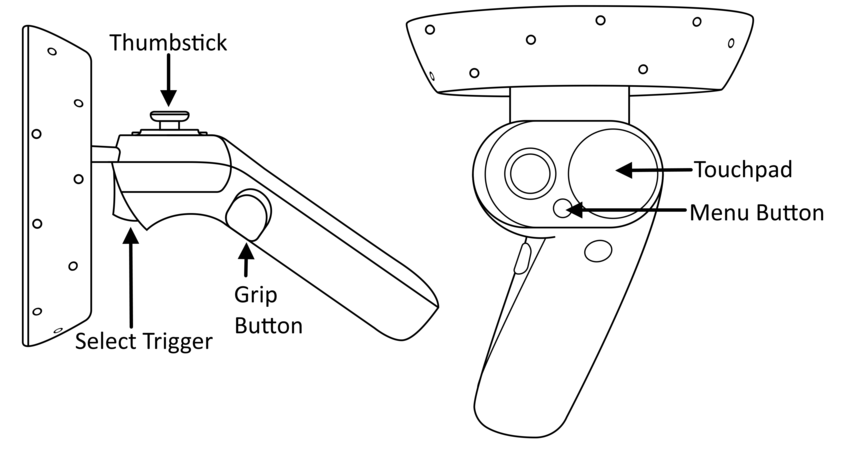
\includegraphics[scale=.35]{hpController.png}
\end{center}

The HP Microsoft Mixed Reality Controllers are wireless controllers that support inside-out tracking, and thus require less initial set up than the other outside-in tracking systems. A lack of required setup time is good, but there are downsides; slightly more latency and the fact that the controllers will not be tracked if the user is not looking at them and they are not in the headset mounted camera view. The controllers are in between the Vive controllers and Oculus Touch in terms of weight and size, and have a slightly lower build quality. They have a trackpad, analogue stick, triggers, grip buttons, and a menu button.

\paragraph{Vive Controller}
\begin{center}
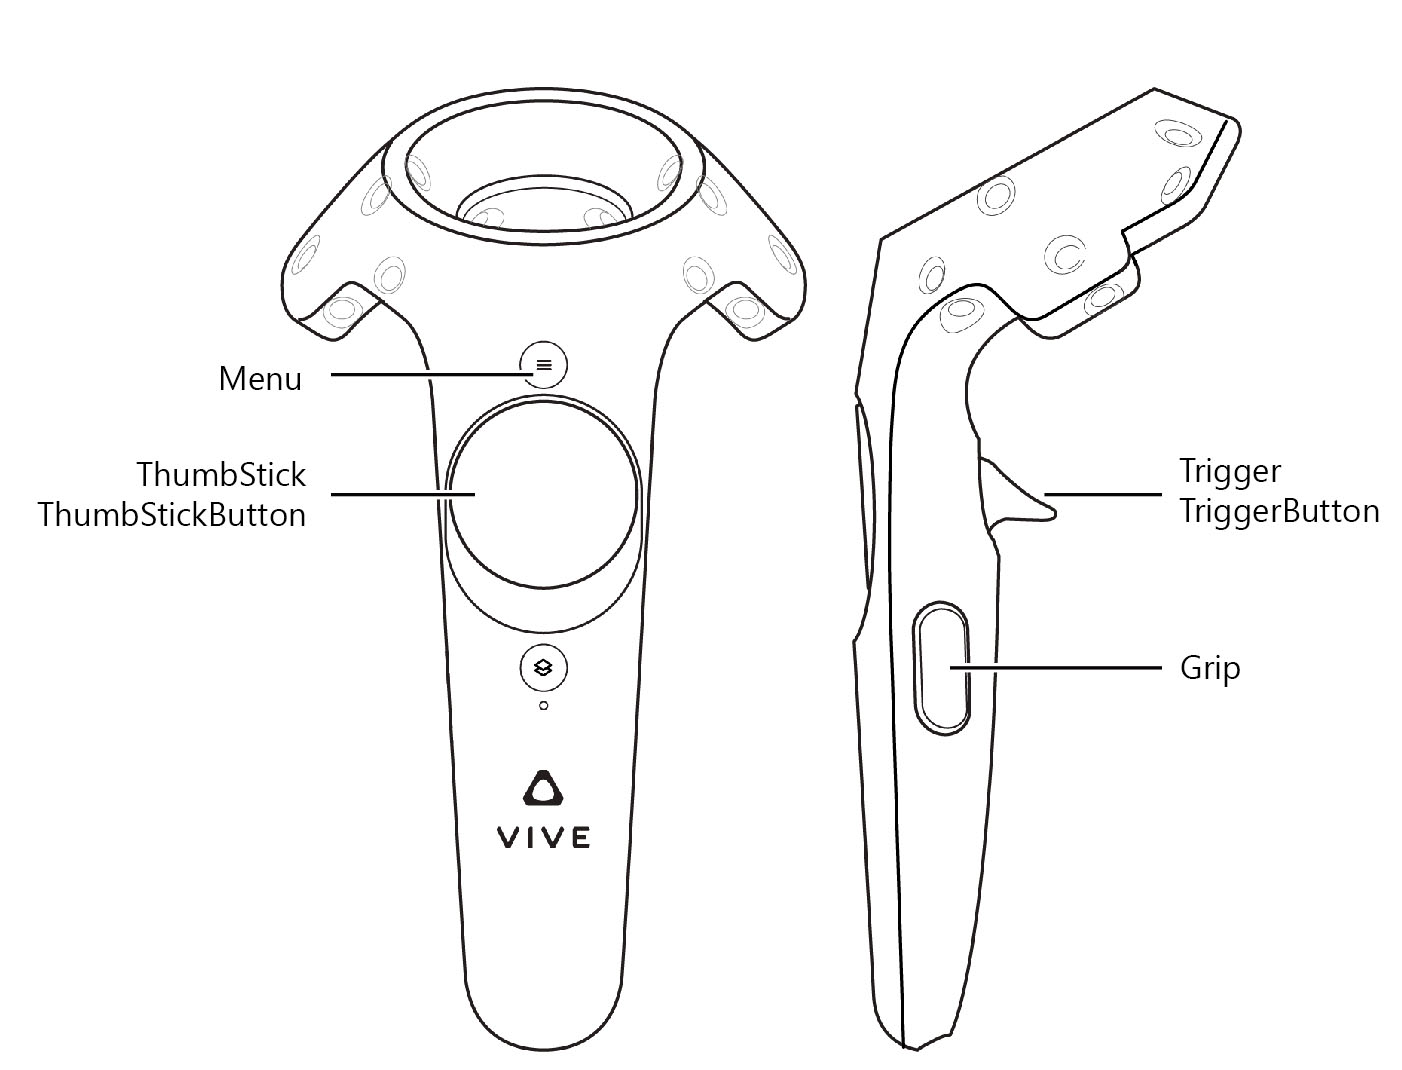
\includegraphics[scale=.20]{viveController.jpg}
\end{center}

The Vive controllers sport wireless controllers that contain rechargeable lithium ion batteries. These controllers have circular touchpad buttons for thumbs, a side mounted grip button, a menu button, a system button, and a trigger on the underside of the controller. Vive controllers are the heaviest and potentially the most unwieldy, due to their overall large size. The controllers also support room scale VR, meaning that the player can actually walk around the room and the camera system will track their position, moving them in the virtual world. 

\subparagraph{Oculus Touch}
\begin{center}
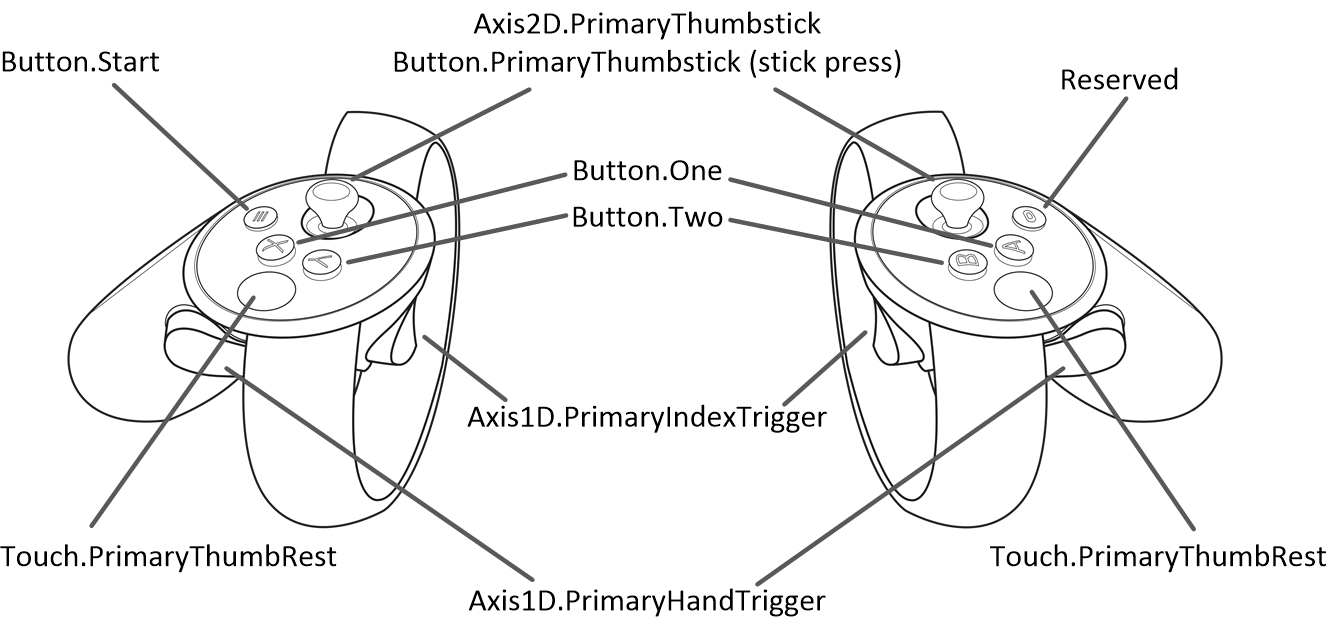
\includegraphics[scale=.30]{oculusController.png}
\end{center}

The Oculus Touch controllers are generally regarded as the best virtual reality controllers currently on the market. They are lightweight and natural feeling, have the best finger tracking around, and have a sleek appearance. One controller is about half the size of a modern gamepad, has two letter buttons, an analogue stick, two triggers, menu and start buttons, a set of buttons on the grip, and a touch sensor for the thumb next to the joystick \cite{controllerCompare}. Having more inputs than any other controller allows the Oculus touch to allow users to have more complex interactions with virtual environments. These controllers are also wireless and require AA batteries. The controllers require the use of a camera sensor and thus an additional USB 3.0 port. During initial setup the user is required to use their motion controllers and the sensors to map the play space, the area that the virtual reality system will allow to player to act in. 

% VRUIs (Virtual Reality User Interfaces)
% VRGUIs (Virtual Reality Graphical User Interfaces)
\paragraph{User Interface (UI)}
User interface is a broad topic and can be applied to many fields, but here we will be talking about UI as it is used in video games and other virtual reality applications. 

% What they are and how they relate to VR
\subsubsection{Types of user interfaces}

\paragraph{Non-diegetic}
The term non-diegetic is generally used in terms of sounds in film, where a non-diegetic sound is a sound whose source is not visible on screen or has not been implied to be present in the action. Non-diegetic UI is generally a UI element or elements that are overlaid on top of the screen to show things like menus, health bars, or other elements that must be view-able and/or intractable by the user. This type of UI is often referred to as Heads Up Display (HUD) in games. Non-diegetic UI does not particularly work in virtual reality, because overlaying something in front of the screen display forces UI elements too close to the eye to be able to focused on.    

\paragraph{Spatial UI}
Spatial UI refers to placing UI "in the world", allowing our eyes to focus on the UI element \cite{unity}. In virtual reality this means that UI lives in the same space as any other objects in the VR scene. This type of UI may need to be scaled according to user position, and may be scaled dynamically. A best practice is to position UI elements at a distance that is comfortable for reading, and scaling the elements based on how far away the user is at any given time. Spatial UI elements are often attached to the camera, so the element will stay fixed in the player view.

\paragraph{Diegetic UI}
Diegetic UI is having elements in the world environment display information to the user. This could refer to things such as in world screens and holographic displays attached to objects. The main difference between spatial UI and diegetic UI is that spatial UI is based on where the user is looking, and diegetic UI is often attached to a non-player object and is independent of player view.  

\subsubsection{Conclusion}
After researching virtual reality headsets, motion controllers, and user interface schemes, I believe that our project would be best served by using the Oculus Rift, the Oculus Touch controllers, and mostly diegetic UI with some spatial UI elements. As of this writing Oculus virtual reality products represent the cutting edge consumer hardware in the field and we would be best served by developing on this hardware. That being said, our client works with HP and the end product will most likely be used with the HP Microsoft Mixed Reality headset and controllers. This means that while we may do most development with Oculus hardware, we must also consider the fact that the end product must also run on the HP headset. At this point I do not believe that this will be a problem, as most VR applications written with commercial game engines, such as Unreal, are headset agnostic. We must be aware of hardware specific features though, and make sure nothing we implement requires a feature of a headset and controller combination that another may not support. 

\bigskip
\begin{thebibliography}{999}

\bibitem{headsetCompare}
  J. Newman and B. Cross,
  'HTC Vive vs. Oculus Rift vs. Windows Mixed Reality: What's the difference?',
  2018.
  [Online].
  Available: https://www.pcworld.com/article/3223202/virtual-reality/htc-vive-vs-oculus-rift-vs-windows-mixed-reality.html
  [Accessed: 10-31-2018]

\bibitem{controllerCompare}
  N. Pino,
  'Oculus Touch',
  2017.
  [Online].
  Available: https://www.techradar.com/reviews/oculus-touch-controller
  [Accessed: 11-2-2018]

\bibitem{unity}
  Unity,
  'User Interfaces for VR'.
  [Online].
  Available: https://unity3d.com/learn/tutorials/topics/virtual-reality/user-interfaces-vr
  [Accessed: 10-31-2018]
 
\end{thebibliography}

\subsection{Stephen Hoffmann}

\subsubsection*{Abstract}
HP is looking for a Virtual Reality solution to help train employees and costumers on their giant industrial printers. The proposed solution is to create a simulated game that will act as supplementary training based on different printer functions and scenarios. This will save time, while also saving money, by providing less in-person formal training at HP’s Corvallis training center. To achieve this goal, our group understands that games require a lot of 3d models. Models define everything you see and interact within a game and simulation. This tech review will go over a range of widely used graphics modeling solutions to find the best fit for this project’s goals.

\subsubsection{Definitions}
\begin{enumerate}
    \item Model - A simulated object that is rendered to appear 3d.
    \item Mesh - The Model's surface skin that is also made up of various geometry, usually triangles
    \item CAD - A file type that holds 3d models, typically used by engineers
    \item Kinematics - creating motion in animations with the use of physics.
    \item UV Maps - The mesh of an object flattened onto a plane, typically used  to paint texture on to models.
    \item Textures - The image the is rendered over a mesh to give the model color, texture, and even shading
\end{enumerate}

\subsubsection{Graphics 3d Modeling Tools}
3D animation software suites cover typically the following features:

\begin{enumerate}
    \item 3D modeling
    \item Mesh UV unwrapping
    \item UV texturing
    \item Frame by frame animation
    \item Bone and Kinematic animation
    \item 3D Sculpting and transformation
    \item Physics and advanced simulation
    \item Programming language based modifications
    \item Rendering[1]
\end{enumerate}

Each feature can consist of a large amount of work depending on the goal, such that individuals can dedicate a whole career on just one of the features.

3D graphics are used for many things, not only games. They are used to create scientific research models, simulations, animated movies, special effects, and much more. The tools that create these models are very complex and require considerable training and experience to use effectively. Depending on the application, producing acceptable results can be achieved in just a few weeks of training, however current industry standards can take an individual years to achieve with one application. So picking a certain tool can impact an entire career in 3d modeling. 
 
Deciding on which tool to use will depend on goals, budget, and the benefits of the tool. I will be reviewing the top three products on the commercial market below, analyzing functionality in respect to modeling, animating, and texturing, while also looking for work-flow speed, costs, targeted audience.

\subsubsection{Maya}
Maya is an industry standard tool for 3d modeling and animation. This product is used by a lot of professional movie studios, as well as game companies. 

Maya also is a fully developed application containing all features found in current competitive applications. What stands out most about Maya is the animation tool-set. Maya supports automatic blending of kinematics to 3d mesh(skin), along with multiple methods to create custom animation bindings. Maya also includes multiple tools and algorithms to transform 3d mesh in multiple ways[1]. 

CAD files are also supported in0 Maya, which is the primary source reference for HP’s printer models. This well allow us to open HP’s custom models and create our own game version, which lowers our team’s time spend on asset creation. Maya does have some noteworthy drawbacks. Due to Maya’s large amount of features and functionality the work-flow can become slow, especially for beginners. However, in spite of this Maya has a quick learning curve due to the features and documentation, including free educational e-books.

While Maya is free for students, Maya is priced at a steep \$3,500 due to targeting large businesses.
\subsubsection{3DS Max}
3DS Max is similar to Maya and is even published by the same Company, Auto-CAD. The primary difference is the targeted audience. 3DS Max is targeted towards designers and artists, such as Game Artists, Architects, and special effects designers. Like Maya, 3DS Max is priced at \$3500, while still being free to use for students. This program takes features away from Maya like scientific simulations and replaces them with stronger features suited for artists. These features include improved modeling tools and improved sculpting tools[1]. 

3DS Max also supports work-flow management by providing linkers to other tools, like Unity, Unreal, and Photoshop. This allows you to work on textures or other game elements within a game engine, while still seeing all updates in 3DS Max load straight-in your game engine. This can greatly reduce overhead in development time due to the costs of always restructuring files and re-importing them in other programs. 

3DS Max also supports custom tools and modifications created by third-party developers to add additional features to games, such as simulated non-physics based cloth movement, hair rendering, and humanoid-type model creation tools with preset animations and layering.

HP’s CAD files are also supported for importing into 3DS MAX.

\subsubsection{Blender} 
Blender is a free open-source 3d modeling and animation tool. Blender is a very capable application that can accomplish anything that Maya and 3DS Max can create. The only issue is that blender is not as developed as other not open-source applications. One potential problem is that Blender does not have native support to import CAD files, which could be a potential issue due to project requirements. Blender also has the largest learning, of both Maya and 3DS Max, due to interface design and a shorter list of overall functionality, but documentation and resources are available. Blender is typically seen as a more manual and involved program for asset creation. 

While Blender has an animation tool-set, it is not as in-depth as the other two programs, missing a few features such as complex layering, and automatic binding of bones. This makes animating take more time, increasing the average time it would take too work on each 3d Asset[2]. 

Blender, however, does support a good sculpting tool-set, that is comparable to 3DS Max, but this does not help in game design due to the nature of need lower polygon count models. Sculpting is usually intended to create highly detailed 3d models that can contain hundreds-of-thousands of polygons[2]. 

Lastly, Blender’s texturing work-flow is fairly straightforward and well supported. The UV unwrapping works intuitively, while also allowing the user to paint directly to the object’s surface. Similar to Maya and 3DS Max, Blender can export UV wraps for easy editing and painting with programs like Adobe Photoshop.

\subsubsection{Conclusion}
Each tool has unique sets of features but ultimately can achieve the same outcome. So when considering we can look at the project's requirements, the tool’s cost and difficulty to learn. 

Starting with Maya, we see high costs, good features, and low learning curve. Along with this, Maya is also a great professional tool for investing time to learn, due to industry demands. 

3DS Max is targeting specifically towards game design, with stronger modeling tools then Maya and a medium learning curve. Again, this is an industry tool, making 3DS Max a good tool to learn. 

Blender is a free and open source program. Blender also has the necessary tools to accomplish the project's requirements, other than having to work around opening HP’s CAD models. Blender also has the highest learning curve and is not a professionally licensed tool. 

Considering the above, 3DS Max stands out in the middle, in terms of project requirements, costs, and learning curve. While costs are high, our team will be able to use it for free, since this project is just a prototype for HP and not a product. If licensing issues a brought up later, then switching to Blender will be as simple as re-saving files in Blender.

\subsubsection{References}
\begin{enumerate}
    \item “Comparison of 3ds Max and Maya,” Autodesk Support \& Learning. [Online]. Available\newline
    https://knowledge.autodesk.com/support/3ds-max/learn-explore/caas/sfdcarticles/sfdcarticles/\newline
    Comparison-of-3ds-Max-and-Maya.html. [Accessed: 10-Nov-2018].
    \item  Foundation, “Features,” blender.org. [Online]. Available: https://www.blender.org/features/.\newline
    [Accessed: 10-Nov-2018].
\end{enumerate}

\subsection{Symon Ramos}
\subsubsection{Abstract}
Virtual, Augmented, and Mixed Reality are growing technologies, each with their own merits and limitations. Many fields and industries are incorporating some sort of virtual immersion. As more studies are performed, an advancement of knowledge in the three technologies will occur, thereby assisting in their development and popularity.


\subsubsection {Project Goal}
 Improve the quality of learning and knowledge of HP's PageWide Web Press equipment and reduce expenses and resources spent by implementing virtual reality based training scenarios.
 
\subsubsection{Introduction}
    %Define what VR/AR/MR are
    In a generation abundant with innovative technologies, Virtual Reality (VR), Augmented Reality (AR), and Mixed Reality (MR) are exciting forms of displaying information that have the potential to change the way we think, improve the way we teach, and revolutionize many fields and industries. 
    %Purpose of VR/AR/MR
    The goal of all three of these systems is to immerse a user in a virtual world that can be interacted with. This can be accomplished with the use of a headset, a set of virtual environment rendering equipment, or even a smartphone. How the virtual objects are displayed within the environment depends on which type (VR, AR, and MR) is being used. All three have strengths and limitations depending on the scenario, field, and availability of one over the others. This document will define each technology and its applicability before evaluating what contrasts it from the other two technologies. Afterwards, the technologies will be analyzed based on their relevance to our project.
    
\subsubsection{Virtual Reality}
    %Define VR, Pro Cons
    VR involves complete immersion into a virtual world. Consequently, because the user is fully immersed, the user fails to sense or identify their real-life surroundings. In addition, some individuals can be prone to a phenomenon known as VR sickness, where the visually induced perception of self-motion can cause disorientation, discomfort, headache, and nausea \cite{2}. One distinct advantage that VR has over AR and MR, however, is the fact that VR can fully immerse users into any given virtual environment, therefore not confining them to the real world they are in (like the classroom or the living room). Instead, as Farshid notes, users can virtually experience going skydiving, visiting famous location, and interacting with exotic animals without having to spend expenses and resources to experience those places \cite{2}. This ability to experience places and objects at any setting makes VR extremely versatile and portable, as it could be used at any location in the world with the same effect.

    The most prominent method of experiencing VR is through the use of VR headsets, which are strapped to the head and, while obscuring vision from the real world, can fully immerse the user no matter what orientation they're is looking at. While most typically associate VR with headsets, there are other ways to accomplish full immersion into a virtual world, such as web applications like the website of the Metropolitan Museum of Art in New York, which provides a substantial virtual tour \cite{2}. Another example would be Google Cardboard as well as other similar headsets that only require the use of a smartphone to create a virtual reality experience. Having readily-available outlets such as those is key to the growth and expansion of VR, as the cost of high-end VR headsets is a limiting factor to its success. 

    VR can be utilized in many fields, such as education and training. Unlike actual real world training, employees of companies who offer VR simulation training can perform modules as many times as they would like to grasp a concept, task, or procedure. Examples of areas where VR technology is improving learning include sales, public speaking, medical surgery, and operating heavy-duty equipment \cite{2}. VR has also been used in education to create more engaging environments that allow students to seamlessly interact with virtual models to teach them concepts in the fields of cosmology, physics, geography, and biology \cite{2}. As VR continues to expand, more fields and industries will find more applicable uses for the technology.
 
\subsubsection{Augmented Reality}
    %Define AR, Pro Cons
    AR, in contrast to VR, is predicated on partial immersion of the virtual world, where virtual objects are displayed in the real world. This allows users to participate in the physical environment while manipulating virtual objects, allowing them to sense and adapt to their surroundings and react accordingly \cite{1}. As described in Farshid's paper in Business Horizons, "actual objects and people cast an information shadow: an aura of data which, when captured and processed intelligently, can offer extraordinary value to consumers" \cite{2}. AR is unique in that it produces information that is readily accessible to users and allows them to perceive digital content in the real world. AR can be generated through many methods such as smart glasses that utilize retinal projection to display virtual data to the wearer's eyes (such as Google Glass or Vaunt by Intel) and (the more commonly used) smartphones \cite{2}. AR layers, as specified by Farshid, can be sensory (which involves the use of sound, video, graphics, or haptics) or only display data \cite{2}.  
    
    One notable example that expresses the novelty of AR is the AR application that Realtor.com has developed which allows potential home buyers to use their phone camera to instantly display information about a certain home, such as last sale price, taxes, and lot size, enabling the user to determine whether an actual market price listing is fair \cite{2}. Another area of life that AR could affect is the act of shopping at grocery stores. With AR-enabled smart glasses or phones, users would be able to quickly and easily be conveyed information about the foods they are looking at, such as dietary restrictions \cite{2}. Driving could also be advanced with the inclusion of AR, which could allow businesses to better display directions and information for possible tourists. Other possible fields where AR could be used are in entertainment, medicine, robotics, and training/maintenance tasks \cite{2}. In regards to maintenance tasks, there are many studies where AR was used as a support mechanism to augment information from manuals when performing tasks on military turrets and aircraft \cite{1}. In the medical field, AR has also been used to guide interactions and improve skills in real-life scenarios \cite{3}. A combination of visual, auditory, and tactile information all assist in rehabilitative experiences for participants. In addition, flexibility was noted as another advantage of AR. These studies have found that having the information displayed directly in the user's field of vision improves efficiency significantly by minimizing the time taken to look back and forth from the manual.

\subsubsection{Mixed Reality}
    %Define MR, Pro Cons
    MR is a type of virtual immersion that is within the spectrum of augmented reality and virtual reality. Often regarded more as a form of augmented reality, MR will augment virtual objects into the real world with the objective of making the object be integrated as seamlessly into the real world as possible. Typically a physical foundation, such as a table, the ground, or specially-designed markers, is used in MR scenarios to convey information. 
    
    By combining aspects of the real world with virtual objects, MR can allow us to experience scenarios that don't actually exist, such as a live video stream of the real world. One notable example of MR is within the field of healthcare, where mannequins that can be used as a physical representation of a person and have augmentations appear on the mannequin to better convey information \cite{2}. Another example that shows the influence that MR can have to technology is the rise and popularity of the app, Pokemon Go, which blends the real world with creatures from an imaginary one \cite{2}. The novelty of seeing your environment within your game, whether it be on the street or on campus or on a hiking trail, can improve the quality of an experience. 

\subsubsection{Conclusion}
    While each of these three technologies utilize virtual objects and environments to display information in a novel and effective way, the differences between the three are notable. VR fully immerses users into a virtual environment of the application's design albeit void of any real world interaction. While both AR and MR have a real world interaction component in their presentation of information, they are bound by the real world and can't fully immerse the user in an entirely different location. 
    Ultimately, as technological advancements are made over time, the fields of VR/AR/MR will grow in both understanding and interest. As explored in this document, there are many applications for each and there are scenarios where one might be favored over the other types of simulations. As research continues, the uncertainty between using one method versus the others will gradually decrease, allowing each to form an identity around particular regions of applicability, such as in education/academics, assembly tasks, and locomotive assistance. 
    
    In regards to the project given to our team to improve the current training method for personnel to learn how to operate HP Web Press printers, using VR to implement new modules was a preliminary decision already made by our client. It's still worth reviewing the advantages and disadvantages to each of the three technologies, however, as it can improve our understanding of why VR is the most applicable option. AR has some merit in that augmentations can be performed on the Web Press printers themselves, thereby displaying additional information (similar to the military turret maintenance example) to assist in task performance, but it ultimately doesn't remedy one major aspect of the project's goal, which is to improve the cost-effectiveness of training personnel. Using AR would still require the allocation of time and resources to use the Web Press printers, whereas in VR, the printer can be created as a virtual object. The argument to use MR also concludes similarly for AR, as both would achieve similar benefits at the cost of similar limitations. Thus, our project goal aligns best with what VR can offer, which ultimately justifies the use of the technology for this project. 


\begin{thebibliography}{}
\bibitem{1}
M. Sidiq and T. Lanker and K. Makhdoomi, "International Journal of Computer Science and Mobile Computing", Vol. 6. Issue 6, June 2017. pp. 324-327.
\bibitem{2}
M. Farshid, J. Paschen, T. Eriksson, and J. Kietzmann, "Go boldly!: Explore augmented reality (AR), virtual reality (VR), and mixed reality (MR) for business", Business Horizons, Vol. 61. Issue 5, 2018. pp. 657-663.
\bibitem{3}
F. Gallun, A. Seitz, T. Vallier, D. Lewis,  "Designing rehabilitative experiences for virtual, mixed, and augmented reality environments", The Journal of the Acoustical Society of America, Vol. 143. Issue 3, 2018.
\end{thebibliography}



\subsection{Stewart Rodger}

\subsubsection*{Abstract}
Virtual Reality shows considerable promise in cutting costs and speeding up training for large machinery like the Page-Wide Web Press. By using a virtual training program, companies can drastically shorten the in person training. Our team will develop a series of virtual training programs for HPs PageWide Web Press product line designed to achieve these goals. In order to achieve this we must have a strong grasp on the the various perspectives and data collection methods necessary to ensure a maximally effective training simulation.      

\subsubsection{Game/Simulation Perspective}
In any game or simulation, there are 3 primary camera positions. "First Person" places the camera on the controlled object or avatar, showing things at eye level. "Third Person" positions the camera behind and slightly above the controlled character. "Overhead" is a camera that is placed high above the scene or level, pointed down. In the image below, A is overhead, B is 1st person, and C and D are 3rd person. [1] 

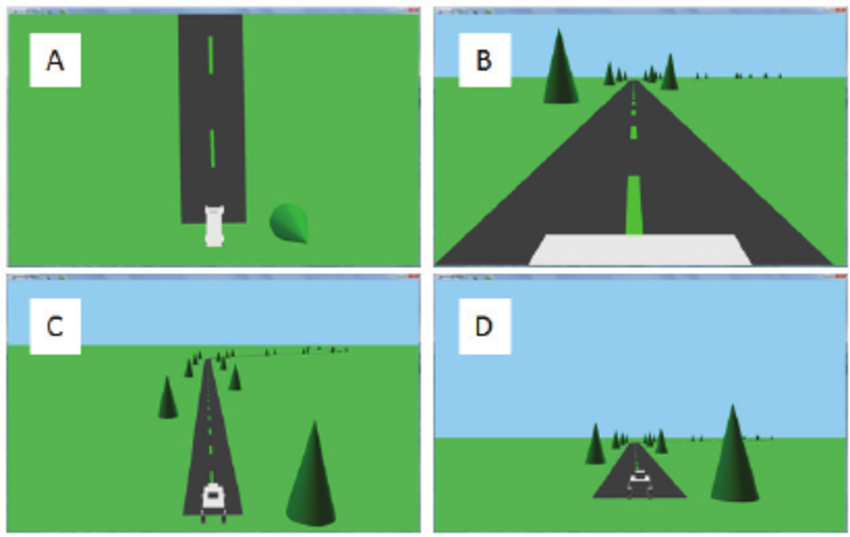
\includegraphics[width=\textwidth]{13o.png}

It is commonly known in game development that the choice of perspective is important to the overall design and "failure to take this particular gameplay element seriously will very likely result in your game controlling horribly, and having a disjointed 'feel'"[2]. Focusing on the camera's value for simulations, there are a few distinct benefits for each option. 

\subsubsubsection{Overhead View}
The overhead view provides a complete view of the scene without having to move the camera. This can simplify the control scheme as the user does not need to worry about controlling the view. The other main benefit of this view is that the user can see everything in the room or scene at once. This allows the user to see cause and effect when interacting with objects that have effects that might be out of view with other camera angles. The downsides is that this is the most dissociative of the camera angles. With overhead view is actions feel the least real, and for complex situations the camera may need to change as it is unable to show the side of a object or machine in detail.

\subsubsubsection{3rd Person View}
The 3rd person camera is the middle ground option. The 3rd person camera still provides a larger field of view than 1st person, while showing the simulation in a more realistic was as the camera is closer to eye level and can properly show the sides of objects. Unfortunately, the 3rd person camera requires the most input controls of the three, and it also is still less immersive than 1st person because the 3rd person allows you to see the back of the avatar being controlled.  

\subsubsubsection{1st Person View}
1st person camera angle is the most immersive of the three [2], with the camera simulating the actual field of view for the controlled character. The downside of first person view is that the the controls can be the most disorienting for users who are inexperienced with virtual environments. First person has a distinct advantage in one area, It is uniquely compatible with a Virtual Reality (VR) headset and control scheme. VR generally does not make 3rd person or Overhead camera controls more convenient or simpler, however it provides both of these benefits to first person view. 


\subsubsection{Data Collection}
An important part of any training simulation is the collection of data. The right kinds of data, collected periodically throughout the test runs, can show what parts of a simulation are flawed, or what parts of the training require more explanation or instruction. However, do to the costs of implementation, "evaluators should focus more on what are those important aspects in game experience (like playability) that we should measure in order to be able to evaluate the game properly, and then select the tools that meet those requirements." [3] There are a few different ways to go about saving user data, the most beneficial are Success/failure counting and Time counting, however there also is an extreme form of data collection through interaction counting.

\subsubsubsection{Success/Failure counting}
Success/Failure counting involves having a system in place to count the number of times a user fails for each task they are attempting to complete. Every time a user, preferably a new test user, is run though the training program, the success/failure count is collected so that we can see what sections were the most prone to errors. The number of failures should be lowered as much as possible though the addition of new objective markers, more or clearer instructions, and the reevaluation of the program to ensure that the success/failure rate is improving. An important aspect of success/failure counting is what to count as an objective worthy of counting the failures for. This results in 2 different methods for success/failure counting, "Basic" and "Hidden".

\paragraph{Basic success/failure}
"Basic" success/failure counting only counts the failure if the user fails to properly complete a objective that they know is a clear objective. For example, if they are provided with a list of tasks to complete, the system will only count if they have failed or completed those tasks. This is the most basic form of failure counting, and it can provide a lot of valuable data about the tasks and the quality of the instructions or simulation. In addition it is relatively quick and cheap to implement. The downsides are that it may miss valuable data by being limited in scope. That is where "hidden" success/failure counting comes in.

\paragraph{Hidden success/failure}
 "Hidden" success/failure counting works as an extension of "Basic" counting.  Instead of counting just the clear objectives, you also have a number of objectives that are not displayed (for example: Did the user interact with the objects in the ideal order, even if that order was not required to succeed?). This provides substantially more data at the cost of development time, as there is no simple list of things to do like with "Basic" counting. This method also cost time later as the data it provides will take more time to sort through. 

\subsubsubsection{Time Counting}
The 2nd main form of data collection is time counting. With this form of data collection the system starts and runs a number of stopwatches in the background and saves the results for specific tasks. A timer begins when the user starts a task and saves when they complete it. The extent of this varies directly with the amount of data the developer is willing to collect and sort through. 


\paragraph{Count total time}
Just like with success/failure, time counting can be applied in a limited capacity, focusing on only the main objectives. In this case the developer can track time from training program launch to success, and track the individual objective attempt times, while keeping development costs/time low. 


\paragraph{Count time between specific actions}
Also similar to success/failure, time counting can be applied to an ever expanding quantity of other hidden objectives. An example could be tracking the time a user spends from when they start the training program to when they first move to learn if they are taking a long time interpreting the instructions.


\subsubsubsection{Interaction Counting}
Interaction counting is exactly how it sounds in the context of the previous two methods. Systems are put in place in the background of the simulation to count every time the user interacts with a specific object or objects. The number of objects that are being watched can vary from 1 to every interact-able object, and clicking on the screen. It is directly expandable to meet the time and cost constraints of development, and it can provide data that the previous methods might miss. Unfortunately, this comes at the cost of a greatly increased data interpretation time. One of the greatest benefits of this method is less about improving user interaction and more about bug fixing. With this method in place, assuming a large enough percentage of objects being tracked, it is possible to recreate the users inputs to find the specific series of events that caused a bug or error to occur. 


\subsubsection*{Conclusion}
For the purposes of this VR training program, 1st person view is the obvious choice. VR will help negate the extra control complications, while providing the most immersive simulation experience we can deliver. For data collection, We will want to use basic form of success/failure and time counting. This will get us the most viable user data while minimizing the amount of extra development time or data analysis time. 

\newpage
\subsubsection*{References}
[1] https://www.researchgate.net/figure/The-four-views-A-overhead-B-first-person-C-third-person-high-D-third-person-low\_fig1\_221474898
\break
[2]  https://www.gamasutra.com/blogs/MichelSabbagh/20150827/252341/The\_important\_differences\_between\_firstperson\_and\_thirdperson\_games.php
\break
[3]  http://tampub.uta.fi/bitstream/handle/10024/79391/gradu03017.pdf;sequence=1

\newpage
\section{Weekly Blog Posts}

\subsection{Nicholas Pugliese}

\textbf{Oct 16, 2018}\\
Progress: We contacted our client and met with him at block 15 to go over initial information about our VR printing project.

Problems: We currently don't all have access to VR headsets in order to get familiar with VR games. Our client told of us that he wanted to approach the development of the VR project as a game development process. As "homework" he told us all to go play VR games to get used to how they work and how tutorials work in VR. We all don't have access to the headsets so we need to get some.

Plans: Get access to a VR headset and play VR games to do our client "homework".\\

\textbf{Oct 21, 2018}\\
Progress:

We met as a team to complete the final draft of the project statement.

Problems:

Out client is currently in Israel and cannot meet with us to discuss the requirements document.

Plans:

We will work together to draft our own set of requirements that the customer will review upon returning from Israel.\\


\textbf{Oct 27, 2018}\\
Progress:

So far our group has been in contact with our sponsor, Tim Holt, about what we should be working on for our group. Tim has said that what we wants us to be doing is playing a few VR games to get ourselves accustomed to the equipment and how VR games are structured vs normal video games. Tim wants to go about making the training application from a game development standpoint and use design philosophies from game design to make a good user experience, specifically taking lessons from tutorials.

Additionally, we also have our outline for our project requirements done and are populating it with our interpretations of what we think the requirements should be.

Problems:

Our project sponsor is still in Israel and cannot devote a lot of time until Monday to helping us with requirements, so much of our requirement document is speculation until our sponsor can get us the training manuals and tell us we are on the right track.

McGrath informed us that the only VR equipment we have access to is in the virtualization lab in Snell hall, which only lets us sign up for hour long blocks. This is fine for us now when all we need to do is play a few games to learn how the tutorials are made and take notes on design. However this poses an issue later in the project if we don't get access to equipment that we can check out for longer periods of time. One hour is not a lot of time to develop games in blocks.

Plans:

After we finish the requirements document we will talk among the group to pick topic that we will write about for our tech reviews since we don't want to accidentally double up on topics.

Also, one of our group members is considering purchasing their own VR headset for personal use. This has the added benefit that we would be able to use it for our group development and not be time restricted. Since two other group member already own VR headsets of some kind, this would speed up development by a lot if we didn't have to use the Snell hall resources to develop.\\

\textbf{Nov 3, 2018}\\
Progress:

Our group was finally able to meet in person with our project sponsor, Tom Holt, at HP to take a tour of the Web Press printers and talk more about expectations of the project. Our group also drafted a requirements document, but it turned into too much of a design document so we created a brand-new document that better fit the "requirements" document description: describing what a solution to the problem statement is required to do, instead of how to do it, which is what our document turned into.

Problems:

Our project sponsor is requiring us to sign an NDA. However, this NDA is not for the entire project, it's just for HP confidential assets such as 3D models and training manuals.

Plans:

Even though we are being required to sign an NDA to use HP assets, it will not get in the way of presenting our project. We will be allowed to create derivative works from the HP-provided CAD files that will not be HP propriety-owned.\\

\textbf{Nov 9, 2018}\\
Progress:

There was not a ton of work for us to do this week. We met in class on Tuesday to peer-review our tech reviews and I got some good feedback about the flow of my paper. I ended up not having to change much from the first draft, since I completed most of it for the first assignment.

Problems:

Our resident game design expect, Stephen, says that we might want to start installing and going through tutorials in the Unreal Engine as it has a steep learning curve. I foresee this being especially challenging for myself as I have very little professional game development experience to my name.

Plans:

Over the remaining weeks of the term I plan on watching Unreal Engine tutorial videos to get up to speed with the rest of my group before the work load starts in Winter term. 

Our team will also work as a group to complete our design document draft, making sure to include the specific user stories that our client request. Last week our client told is that these users stories should include the proper sound ambiance as what is found in the actual R\&D location at HP.\\

\textbf{Nov 16, 2018}\\
Progress:

This week there was not a lot of things for us to do. Last Friday we finished our Tech Reviews and this week in class we talked all about design documents, and got lectured at by McGrath about using spellcheck.

Problems:

Our client has not been very attentive in answering emails. We sent him a progress update for our documentation last Friday and we still have not received word back from him. I also do not feel inclined to come to Thursday lecture if I have to listen to McGrath belittle me as a student for having "poor writing."

Plans:

For the coming holiday weeks we are going to work on the design document to finish it up. We got information from Chris that said each section of the document needs to be 500 words or longer, to ensure that we only write about things that have content.

Also for next term during the design phase we are going to try and set up a weekly meeting with our client so that both us and him feel like we have a good understanding of the project moving forward.\\

\textbf{Nov 22, 2018}
Progress:

We have not made any progress this week on our project.  We did receive an email from our project sponsor Tim about the state of the NDA we have to sign to get access to the source files. We sign it on our own and bring it to the HR person at HP that oversees Tin's department. Again: this NDA only coves the base .stl CAD files that we will be using as a reference, and does not extend to our project in any way. The final project will not be secret and we will be able to call it our own and present it at the career fair.

Problems:

My tech review has not yet been graded so I am unable to review feedback about my writing to apply it to my sections of the design document.

Plans:

This weekend we will finish the design document making sure to follow the ISO standard properly this time. I will ask another one of my group members about their feedback for their tech review in order to better prepare myself for my sections of the design document. \\

\subsubsection{Winter}

\textbf{Jan 11, 2019}\\
Progress:

So far we have contacted McGrath with a request for VR headsets, contacted our client Tim about setting up a weekly meeting with him to go over progress, and set up a weekly meeting with our illustrious TA chris for another progress report.

Problems:

There was some pushback with McGrath when we requested hardware. When we requested two headsets for our group Kevin replied with "I’m sorry, did you really just ask for \$2400 in headsets with a straight face?" This reply did not sit well with our team and were frustrated at first, before McGrath replied again with a bit nicer of a prospect for our team.

Plans:

Wait for Tim to reply and have our first meeting with him to figure out the best place for us to begin developing. Additionally, wait for our headsets from OSU to get in.\\

\textbf{Jan 18, 2019}\\
Progress:

I have installed and done some unreal tutorials with another group member to get myself up to speed. Additionally, our group has received 3 VR headsets to use for development. We have setup a Kanban board for organization are are about to really start our level design.

Problems:

Our project sponsor, Tim, has not yet replied to our email about setting up a weekly meeting. It has been 8 days. I will send a follow up email monday morning in the hopes that he will see it while at work and not let it get bogged down.

Plans:

If Tim still hasn't replied by monday, I will take our group to the webpress to take pictures and measurements to start blocking the levels out in unreal. Aside from that, we will work together on dividing out tasks on the kanban board for completion, as well as brainstorming new tasks.\\

\textbf{Jan 25, 2019}
Progress:

We were able to get our clients response! Tim came to campus today and we're discussed concrete designs for the VR application. we also setup a recurring meeting with him on Fridays.

Problems:

No problems this week.

Plans:

Kyle and Symon checked out the computer graphics lab in batcheller hall for our use of development. each computer has a 1080ti and the unreal engine we we will be using those for development. We have a sample project in a git repo ready to go for additions, so all we need is to start development. we picked Monday afternoons to work for a couple hours together. \\

\textbf{Feb 1, 2019}
Progress:

Ground breaking week for us. We have a working emergency light object blueprint in unreal, a rough 3D model of the press that Stephen made by hand, and a working user interface.

Problems:

When Stephen and I went to HP to meet with Tim to take pictures of the press, the 3 of us got scolded by the floor manager of the web press for not wearing proper safety gear and for not informing them we would be around. Tim in fact did email that person's boss that we would be arriving, the boss just didn't relay that information to the floor manager. This lead to an awkward accusatory conversation where the floor lead said multiple times "we can help you, you just have to help us help you." In the end he was actually really receptive of our mission (even though we neglected to tell him we were taking pictures of his machinery) because it would cut down on the physical training he would have to put his operators through.

Plans:

The floor manager suggested that we could take some of the training classes that HP offers in order to more familiarize ourselves with the press and its operation. Tim is looking into if that is feasible for our timeframe.

Other than that we will continue the work! I continue to add items to the trello board as people tell me what is completed and we get closer to a functional simulator.\\

\textbf{Feb 8, 2019}\\
Progress:

We have fully integrated all of the 3D models of the web press into our VR landscape. We also have added supplementary models to make the space feel more at home, like an actual warehouse aesthetic with rafters and lights, as well as computer desks and rolls of paper.

Problems

Not really a lot of problems this week. We spent a lot of good time developing and made good progress. Our client forgot our meeting today, but it wasn't that critical so we really didn't miss much.

Plans

We drafted up ideas for the VR tutorial we plan to include alongside the training application. These tutorials will teach the user how VR works (looking around, pointing the controllers, teleporting, etc) in an office setting that we plan on adding to the press room. I am going to take a stab at modeling it so I can say I contributed more than just organizational work to this project.\\

\textbf{Feb 15, 2019}\\
Progress:

We have laid the groundwork for all of the specific scenarios we plan to implement by adding the level geometry and 3d models to our main map. There is a new office space to be used for the tutorials.

Problems

not a lot of issues, just scrambling to get ready for alpha release

Plans

implement the first scenario for replacing a printhead from the printbar. once that is done we will have met our clients expectations. we plan on writing the scenario functionality to be easily scalable to be used for other module s since we want HP to be able to turn this into whatever they want.

we are also planning on having a printable PDF that showcases how to use the VR controls for people that have never used VR before. we are going to include the PDF as a poster in the environment so the user can view the controls without removing the headset.\\

\textbf{Feb 22, 2019}\\
Progress:

Tutorials for looking around in VR, teleporting in VR, and interacting with grabable objects are now done. The next step is to complete the unreal blueprint for the training scenarios. Stephen is working on this today and tomorrow and we will finish it on Sunday.

Problems

Not a lot of problems this week. All good development done. We are on track.

Plans

We are getting together Sunday afternoon to implement the final push for alpha release on Monday. We are updating the progress report as we go (currently up to 10 pages) so we don't have to have a scramble at the end of the day tomorrow, which is nice.\\

\textbf{Mar 1, 2019}\\
Progress:

Everyone in our group is finally not sick this week and can work again. Stewart is working on making sure the tutorial works with the HP headset, Kyle and Stephen are working on the training blueprint for scenarios (as well as fixing the bugs I introduced, oops), and Symon and I are thinking about what should go into the voiceover part of the tutorial.

Problems:

Tim was sick this week and didn't get to see what we had done, which is fine for us since we were sick the previous week and also didn't do much besides talk about what needed to be done. However, we did write our progress report draft well (according the the peer reviews I have received), so it wasn't wasted time at all.

Plans:

Finish the last goals of the project such as actually make the training scenario, set up the voiceover and on screen text, polish everything the the warehouse environment, and just generally keep working on the things we hashed out in previous weeks.\\

\textbf{Mar 10, 2019}\\
Progress:

It's actually kind of serendipitous that I forgot about my progress report... Because we finally have a basic scenario done now! Stewart sent me a pull request for it a few hours ago. Its a training scenario blueprint for replacing printheads in the WebPress.

Problems:

Stephen has been unable to work for the past few weeks due to his having the flue. Today he also discovered he is allergic to the antibiotics he was prescribed and had to go to the hospital. Yikes! He seems okay from the messages he sent, but we've been down a developer for the past 2-3 weeks. Additionally, we were not able to meet with Tim this week and he is going on vacation next week so we will probably only be able to show him things after the end of this term. Not to worry though, we went over with him what beta release should look like and he agreed that having one scenario done would be plenty.

Plans:

Polish the hell out of things! We want it to look and act nice for expo. Now that we have a basis of what to work on (the scenario blueprint) we can easily expand it into printheads and e-stop buttons. Anything we want, really.

\textbf{Mar 15, 2019}\\
Progress:

Stewart pushed the final changes to the scenario on Friday. We now have a working training module that shows someone how to remove and replace a printhead from the webpress. When we last talked to our client, this was what he was hoping to accomplish with the project: to be able to demonstrate to upper management that using VR could be an important teaching tool that can save HP time and money.

Problems:

Even though everyone has told me that we are where we need to be in terms of progress on the project, I can't help but shake that feeling of dread as we come closer to the deadline. I really don't want to fail this class and need to take another year of school. I know that happening in extremely rare and most everyone that puts in work will pass. We certainly have put in work, so bare minimum we will pass. The important thing is that we did what we said we would do, and our client likes it.

Plans:

All we need to do for this term is to record the video. Everything could be upgrade once or twice over in terms of visual appeal and style, but I assume that is what we will be doing most of next term to prepare for expo.

\subsubsubsection{Spring}

\textbf{Apr 5, 2019}\\
Progress:

After the class today we met and talked about what final details we needed for code freeze. Most of it boiled down to reorganizing the project folders to be nice. The biggest thing we need to do it wait for a reply from our client to schedule a demo for him to get his feedback about what things we need to change.

Problems:

No problems as of yet.

Plans:

Review the documentation to make sure no revisions are necessary. We don't anticipate needing to do much (or any), but we are still going to check.\\

\textbf{Apr 12, 2019}\\
Progress

We have added the last bits of polish, fixed the controllers (the HP plugin was broken, so we now only rely on the steam API), and started the user guide for code-freeze.

Plans

Continue to try and build the executable and draft the user guide. My task is also to review the requirements and see if anything has been updated.

 
Problems:

Still no reply from Tim yet. Hoping he stops being AWOL in time.\\

\textbf{Apr 19, 2019}\\
Progress:

Nothing new since last week.

Plans:

Continue doing assignments as they come.

Problems:

Still no client verification, but I talked to Kirsten and she told me to submit it anyway because it's out of our hands.\\

\textbf{Apr 27, 2019}\\
Only new thing to report this week is that we got client verification finally, as well as finished our poster. \\

\textbf{May 3, 2019}\\
Nothing new to report this week.\\

\textbf{May 10, 2019}\\
Nothing new to report this week.\\

\subsection{Kyle Tyler}

\textbf{Oct 19, 2018}\\
This week was relatively slow in terms of progress on the project, but our group did move forward in the planning stage. We turned in our individual problem statements and then worked together to complete our group final problem statement. Everybody had a solid personal problem statement, so we really just took the best parts of each and combined them into a document we were all happy with. Another thing we did this week was get started on our requirements document. Lastly, we had our first meeting with our group TA.
One problem I foresee is that our client is going to be out of town for some of next week, and may not be available to go over our requirements document. Our group is also hoping to get access to VR headsets so that we can familiarize ourselves with the technology (per our client’s request), but are not sure how likely that is to happen soon.
Our plans include finishing up our requirements document, meeting with our client, and taking some time to learn Unreal Engine.\\

\textbf{Oct 26, 2018}\\
This week has been a little slow in terms of overall progress on the project. Our group is mostly dealing with creating a good requirements document that will serve as a good base from which to move forward on the project. I thought that the document would be a little simpler and less work than it is turning out to be. I'd say that is because this is the point where we are starting to dive deep into what is really going into this project, so there is a lot to flesh out. We plan on finishing the requirements document this weekend. After that I will be starting on the first draft of my tech review.\\

\textbf{Nov 2, 2018}\\
This week has been kind of a crazy one. Between midterms in other classes and fairly large writing assignments in this one, there hasn't been a whole lot of downtime. That being said, a lot of progress has been made this week. Our requirements document was turning out to be more of a design document than a requirements doc, so we had to start from scratch and create a more concise document. I made a tentative gantt chart to go along with that. We also worked on tech reviews, which turned out to be more fun and interesting than I had anticipated. I looked at virtual reality hardware, so ending up learning a lot about the differences between VR systems.
Our plans are to finish up the tech reviews, do peer reviews, and come together to create a final tech review.\\

\textbf{Nov 9, 2018}\\
This week was a relatively slow one, for this class at least. We did in class peer reviews on the tech reviews, which I found to be pretty helpful. I didn't end up having to change a whole lot of my paper, but getting more eyes on it helped, and it was interesting reading other people's work. Our group is starting to think about design document, which we kind of got  a head start on due to accidentally starting it instead of our requirements doc a couple weeks ago.
So the plan is to work on design and keep learning about tech in our spare time (VR, Unreal).\\

\textbf{Nov 16, 2018}\\
This was a pretty light week. There was nothing due this week, but we did start thinking about end-of-term stuff, like the design document and our progress presentation. So far there are no real worries, just have to continue knocking things off the list.
We contacted our client in the last week, to see if he wanted to meet again soon, and haven't heard anything back yet. I have also been meaning to work more with Unreal engine this term, but time hasn't really allowed, so hopefully I can brush up on it over Winter break!\\

\textbf{Nov 23, 2018}\\
This week we started looking forward to what all needs to be done before the end of this term. The group has met to talk about the design document and started working on it. It turns out that when we wrote our first draft of our requirements document it was basically a design document, so we have a good head start on this assignment. We will continue to work on that this weekend. Our client also got back to us about the NDA we need to sign in order to see HP's CAD models. It looks like we can all sign it and get the paper to him as soon as is convenient.\\

\textbf{Jan 11, 2019}\\
This first week the project did not move along all that much, mostly because we are all settling into new schedules and figuring out what our workflow is going to look like. The group is also getting more familiar with Unreal Engine, which is a project in and of itself. For my part I am learning more about the Unreal visual scripting system and level design tools. We also contacted Kevin about VR hardware and that should be arriving early next week. Lastly, we contacted our client in hopes of meeting up next week.
There were no real problems this week, but it is clear we need to get organized and start splitting up work.
Plans include meeting with our client next Monday, having our first TA meeting with Chris, getting version control setup for our project, and prototyping a rough level to test our newly acquired VR hardware.\\

\textbf{Jan 18, 2019}\\
This week we made a little bit of progress. We got hardware, more than we had thought we were going to get. Three HP headsets for me, Nick, and Symon to use because Stewart and Stephen have their own HMDs. Having those allowed us to play around with VR and get more comfortable with designing for the medium. I have also been using a lot more Unreal Engine, and am finally working my way up the steep learning curve associated with the tool. We also made a group Trello, so we can more easily track tasks, see what needs to be done, and who is doing it.
As for problems, there are a couple. We still haven’t heard back from our client at HP. We probably should have sent him a follow up email earlier in the week, but since it is Friday I think it is best if we wait to do it Tuesday morning (Monday is a holiday) to lower the chance the email gets lost in the abyss. I also am a little concerned with the amount of progress we have made on the project itself, which is little to none. We are all settling into the term, are busy, and learning new tech, but I think we need to make some serious headway in the next couple weeks and have a working prototype as soon as possible.
This next week the plan is to begin work in earnest on the project. We need to get a basic level up and running in Unreal and make sure we can use the VR headsets with our project. We also need to meet with our client and go over what the rest of development will look like. I think we will be okay, but we do need to start making some progress.\\

\textbf{Jan 25, 2019}\\
This week we made some good (mostly organizational) progress on the project. We set up more of the Trello board, which we are using to track tasks, got a shared Unreal project in Github, and met with our client to talk about the project. Our meeting with the client went really well, and he gave us some good ideas to bring into our work going forward. He gave us some CAD model files to look at, and suggested that we meet again at HP to get a sense of scale of the Web Press room so we can scale our prototype correctly.
There were not a whole lot of problems. The only real problems I foresee are that it is hard to get together and work on this project, and that I and the others in our group have a pretty full class load, so we aren’t spending as much time on this project as we would like.
We plan to meet next week to develop together, and to get a prototype level up and running so that we can show Tim at our next meeting.\\

\textbf{Feb 1, 2019}\\
This week was a productive one for us! We all got involved in development and started really getting into the swing of things. There is now a working prototype level with a rough training scenario, a menu UI system, and a model of the press currently being made. These are essential pieces, and it feels good to have made progress on them. We showed what we have now to our client today (Friday) and he liked what he saw.
No real problems came up this week. We set a goal for what we would have done this week and we actually finished all of that!
Next steps are going to be to polish the press room we have now. An important piece of VR is immersion and creating the sense of inhabiting a real space, and that is going to take some design work to fill out the level. We also want to make a training room that will teach first time users how to use VR. This is something our client clearly cares about, and would be a good way to teach users the basics of our application.\\

\textbf{Feb 8, 2019}\\
This week we made some pretty good progress. We got a main level up and running, so now our room is not just a sad little test map. Stephen modeled the web press and that is in the project now, and it looks great. I also did a lot of project cleaning (a game project file structure gets messy quick with a lot of people touching it).
There was only one small problem this week, and it’s that Stewart’s UI implementation was hard to merge with the main project. Something about his personal development environment wasn’t compatible with our project. That whole situation is still in progress.
We plan to keep polishing the main level and light scenario. Immersion is really important to us, so we want to spend a lot of time making sure the place feels real. We also want to implement a training room that will help introduce VR to new users.\\

\textbf{Feb 16, 2019}\\
This week we made good progress on the project. We have continued to polish the level, added more interactions, and integrated the menu UI system to the main project. There have also been improvements made to the web press model to make it more realistic.
There were no major problems this week, mostly just trying to get as much done as possible and checking things off the to do list.
Our plans for this next week are to try to complete a whole training scenario from start to finish, complete with UI. We also hope to start work on a tutorial room to teach users the basics of our app.\\

\textbf{Feb 21, 2019}\\
I’m doing this a day early because I will be out of town all day tomorrow (Friday). This week was a bit slower than other weeks, but a lot was still accomplished. I know personally I wasn’t able to get as much done on the project this week due to other classes, but the team as a whole made some good forward progress. We got the printer model updated, and also started implementing functionality for both the tutorial and the main training scenario (replacing an overheated print head).
We ran into a little problem merging different versions of the project. Stewart has been primarily handling UI and tutorial stuff, and the merge broke some references to updated assets. Nothing major, but a reminder of the dangers of working on different versions of the project.
This next week we will continue to work on the tutorial and main training scenario. We want to make sure that these work and can be tested from start to finish, even if they are not particularly polished yet.\\

\textbf{March 1, 2019}\\
This week was pretty good. We made progress on the tutorial section and it is essentially feature complete. It is a little buggy, but we are happy with the overall flow of the tutorial at this point. More progress was also made on the main training scenario. The interaction with the printer pieces was polished and all that needs to be done is to hook the printer state up to some UI elements.
Progress this week was good, and the only problems we had were just that a couple of our team got pretty sick this week. Luckily we were still able to achieve a lot of our goals for the week.
Plans include: hooking the main training scenario up to UI, polishing user interaction mechanics, and improvements to the 3D environment.\\

\textbf{March 11, 2019}\\
Sorry this is late!
This week some good progress was made on the project. We were able to get both the tutorial and main training scenario completed. They are not totally polished, but the scenario can be ran from start to finish. The warehouse environment also got lighting and material improvements, trying to make the space more readable and realistic.
Problems this week are just that I wish I had more time for the project, but other classes are destroying me! We also have a sick team member, but we have been able to keep up.
Our plans include polishing the tutorial and training scenario, more environment polish, and doing end of term documentation.\\

\textbf{March 15, 2019}\\
This week no huge steps were taken on the project, as we are all pretty much swamped because of finals stuff. We have mostly been talking about what all we need to ensure we are set for beta release, and the consensus is that we are basically there. All of the core elements are in place, they just need more polish which will come at the start of next term.
This week I had a version control problem. I had made some new materials and revamped the lighting, and for some reason my changes were lost. I think I wasn’t on the most recent version of the project, something just went wrong somewhere. Not a huge deal, just need to put in more time to redo that.
Our plans for this next week are to add some finishing touches to the project, finish our write up, and record the progress video on Monday.\\

\textbf{Apr 5, 2019}\\
This week we set up group meeting times, set a meeting with our client for next week, and set TA meeting times. We also talked over what is top priority for code freeze, and we decided to focus on integrating sound, writing a good user guide, and making sure that the full scenario can be completed easily when running the app as a standalone executable.
We plan to work on these things over the next couple weeks and then continue to polish the project for expo. I personally am interested in adding a couple touches to make the experience more fun to show off to users, because I see that people really like to play around in VR, and that’s the kind of stuff I like to make. We have really hit all of our requirements, so I want to take some time to implement things from our “wishlist”.\\

\textbf{Apr 12, 2019}\\
This week we got a lot done! There were some bugs related to controller inputs that had been plaguing us for a bit, but I found that it was just due to some incompatible plugins in Unreal. We also added sound, cleaned up the project file structure, added in more interactable objects, and added tooltips to the controllers.
We still need to put together instructions for the graders, and build and test an executable version of our project. Unreal is weird, so I’m hoping that is easy, but I really don’t know yet. The combo of Unreal, the SteamVR API, and the HP headset has kind of been a headache to develop for.\\

\textbf{Apr 19, 2019}\\
Not a lot happened this week besides preparing for code freeze. There were a few issues that came up when we were trying to build an executable from our project, but nothing that was too much to handle. That got all submitted in time, we verified some info for expo.
We are having a little trouble getting a hold of our client. He has been relatively unresponsive. He did reply a couple days ago and apologized for the slow reply and that he would look over the documentation soon. Besides this, everything is coming together! We are looking to polish up a couple things before expo, maybe add some fun interactions and objects for the live demo, but that’s about it.\\

\textbf{Apr 27, 2019}\\
This week not a whole lot happened. There are a few things we still might want to implement in the project, but nothing that really needs to go in before expo. We really just plan to go through it a few times to make sure there is nothing we need to streamline more for the live demo.
Something I want to do is make a level that doesn't have any event logic tied to it, so we can just have users look around and poke at the environment. It might be cool to put some more fun objects in to give them something interesting to mess around with. The live demo isn't strictly necessary, so I want to make sure it is enjoyable for users to mess with.
This week we also got together a final draft of the poster for review, and will send that off for printing as soon as it is okayed.\\

\textbf{May 3, 2019}\\
A little late on this one, sorry! Not a lot again happened this week. We finished up our poster, got model release forms turned in, and are mentally preparing for expo. Not a whole lot left to do, we are looking good!\\

\textbf{May 10, 2019}\\
Not a lot again this week. We went to class and got filled in on most everything we needed to know about expo. We are ready!!! There is a list of stuff we know we need, and have backup plans in case anything falls through. \\



\subsection{Stephen Hoffmann}

\textbf{Oct 19 2018}\\
  \textbf{Progress:}
  We meet as a group and completed our problem statement, as well as decided how to do the next assignment. We also met our ta.

  \textbf{Problems:}
  Team Member still want access to VR headsets, as per client request. We are still figuring that out. The client in out of the country for the next week.

  \textbf{Plans:} 
  Figure out the VR gear situation and work together too complete the requirements document.\\

\textbf{Oct 26 2018}\\
\textbf{Progress:}
We have each been completing sections of the requirement document, with updates nearly every day. We each divided the outline of the document as fair as possible. Along with team members are starting to look into downloading the Unreal Engine and start learning. We have also discussed possible tech resource topics, that would be interesting based on each owns interests in the project. For example, I will probably be looking into which tools to use for recording, editing, and layering sound files.

\textbf{Problems:}
We won't have time to let the client review the draft, due to him being on vacation, but this can be done later. The extended due date also helped with other class requirements and our own planning.

\textbf{Plans:}
Have the documentation ready to go before submission date. I will also start training on Unreal, as well as refreshing myself on other tools I will know I need, such as Maya, Reaper(Sound Studio), and Photoshop.\\

\textbf{Nov 2 2018}\\
\textbf{Progress:}
On Friday we met out client, Tim, and got a tour of HP's printer press and he shared some ideas of what he would like to see. We got good notes and a better idea of our scope. However, Tim does favor a large goal, so we have to stay on top of him when he gets excited and talks about what he wants to see in a couple years.

\textbf{Problems:}
Tim still wants us to be able to have headsets at home to play with. He understand that McGrath wants us to wait, so he will try and ask around HP in attempt to get us a couple now. He doesn't necessarily want us to start, but learn the interface of existing games and feel and respond in VR. This is due to the nature of many team members never trying VR.

\textbf{Plans:}
Tim wants to start meeting weekly now that he is back from Israel. He also invited us to work at HP once a week for about 2 hours if we wanted too. Looking forward, we will start to focus on more formal goals when talking to Tim, which will lead to hopefully the planning and design of our first scenario.\\

\textbf{Nov 9 2018}\\
\textbf{Progress:}
We finished up our tech reviews and looked over each others, as well as doing peer review with other teams. I have started training on Unreal, and we emailed the client on if he had updates for us concerning test files, NDA, and getting a training manual.

\textbf{Problems:}
We still are waiting on the training manual so we can finalize a strong plan on specifically what training scenario we will plan for. Hopefully the client will give us this next week, our design document will need to rely on it.

\textbf{Plans:} 
keep in touch with the client and plan to meet hopefully sometime next week at HP. We all also agreed to start actually learning unreal instead of just thinking about it, hopefully we all have time for this.\\

\textbf{Nov 16 2018}\\
\textbf{Progress:}
This week we talking about starting the design document and what we need to do with the one we already started to ensure it meets the requirements.

\textbf{Problems:}
We have been emailing Tim our client however we have yet to receive a response in two weeks, hopefully next week....

\textbf{Plans:}
Keep emailing Tim every 2 business days so we can get things moving forward. Start working on the design document.\\

\textbf{Nov 23 2018}\\
\textbf{Progress:}
Working on the design document, got email back from client requesting a NDA, hopefully meet with him next week. It was a short week due to holidays so progress is limited.

\textbf{Plans:} 
Sign the DNA and meet client so we can get access to company CAD models to start project. Finish Design Document by due date.

\textbf{Problems:} 
Weekend plans with the holidays made it so we couldn't meet client this week, but overall it is not that important.\\

\textbf{Jan 11 2019}\\
\textbf{Progress:}
emailed Mcgrath for hardwarew and he ordered some hp headets. Emailed Tim to let him know when we are available to meet at HP. Everyone is now getting together and learning unreal.

\textbf{Problems:}
Waiting on CAD files and documents from HP.

\textbf{Plans:} 
Hopefully get CAD files and training docs to flesh out a more detailed task list of goals.\\

\textbf{Jan 18 2019}\\
\textbf{Progress:} 
Found out where to get most of our art assets for free, so we will not have to make a lot of generic office furniture and supplies to create our 3d world. Everyone is still working on unreal and getting stuff put together. We also now have enough headsets for everyone in the group which is awesome.

\textbf{Problems:}
no word from client. This isn't holding back on the short term as we learn tools and get things together, but will hurt long term goals if he doesn't reach out soon.

\textbf{Plans:}
keep trying to get in touch with out client. Keep playing in unreal and starting building our test environment. Setup up git with Unreal, start creating agile tasks and weekly outlines.\\

\textbf{Jan 25 2019}\\
\textbf{Progress:} 
Finally met with client, got more detials and quest requirements. Got some CAD files to work with. Found out how to get all the other models we should need. Level design is coming along. Unreal is becoming more familiar.

\textbf{Problems:} 
Still need to get repo running, should have that done soon.

\textbf{Plans:} 
Get Unreal repo, make sure everyone is on the same page, and start getting user stories done.\\

\textbf{Feb 1 2019}\\

\textbf{Progress:}
Completed rough draft 3d printer models. Me and Nick also met Tim at HP on Wednesday to take photos and gather more information. We also met team as a group on Friday and discussed team progress and goals before the next meeting.

\textbf{Problems:}
Cad files to large for my system memory to import, causing crashing after about 45minutes of attempting to upload. Ending up wasting a lot of time with this. Instead, I am freestyling the models based on images rather than cad models.

\textbf{Plans:}
Finish the models and animations this weekend so we can start too implement printer features in VR.\\

\textbf{Feb 8 2019}\\
\textbf{Progress:}
Models are done and in the game engine, we have built a factory environment, also created and added models that are found at HP. 

\textbf{Problems:} 
some of the models doors have pivoting issues, will need to edit this. UV mappings in some Sketch-up models are also causing texture issues. 

\textbf{Plans:} 
I plan on fixing the 3d pivot issues this week, and redo the imported Sketch-up models UV wrappings too allow proper texturing. Start the tutorial features with group and specific in game printer features, like inserting new printer heads in the printer.\\

\textbf{Feb 16 2019}\\

\textbf{Progress:}
Fixed all model issues, met with Tim and review the level of detail of models and his thoughts on what we have.

\textbf{Problems:} 
No real problems at the moment just good overall team progress.

\textbf{Plans:} 
Meeting on Sunday too work on alpha stage requirements. Should be getting a good sprint in to show off new features to Tim next week.\\

\textbf{Feb 23 2019}\\
\textbf{Progress:}
Figuring out how to integrate Stewards UI into printer scenarios.

\textbf{Problems:} 
Been out with the flu since Wednesday and still recovering, hadn't been able to work as much as I would like.

\textbf{Plans:}
Finish printer scenario by next week with team.\\

\textbf{Mar 1 2019}\\
\textbf{Progress:} 
Debugged blueprints to fix problems concerning printer interaction. Taking printer pieces out had three bugs and they are now taken care of.

\textbf{Problems:} 
No real issues. Client was sick so no weekly meeting, and possible issue with McGrath strongly recommending not to do a live demo during expo.

\textbf{Plans:}
Get doors functions in a way that feels good in VR. The doors are function kinda like trunks of cars and open upward by rotation. It might get tricky figuring out how too rotate it according too user hands.\\

\textbf{Mar 8 2019}\\
\textbf{Progress:} 
Me and Symon got together and recorded all the voiceover and sound effects we need. I also edited and compiled all sounds into files for unreal

\textbf{Problems:}
Nothing to much, the client is still sick and is then going on a vacation next week, so we wont see him for a while.

\textbf{Plans:} 
Finish blueprints for player experience. \\

\textbf{Mar 15 2019}\\
\textbf{Progress:}
finished blueprints for printer doors. They don't quite have the animation I wanted, but they are at least functional.

\textbf{Problems:} 
No Tim for the rest of the term, but we do have good progress and he know we are on track.

\textbf{Plans:} 
Meeting on Monday to record video and finalize documentation for the term.\\

\textbf{Apr 5 2019}\\
\textbf{Progress:} 
We meet as a group multiple times and discussed our plans and goals going forward into code freeze.

\textbf{Plans:} 
Hopefully meet with Tim next week and decide on last minute additions and approve our revised documents. I will also be adding better animations too doors, and fixing various UV wrapping issues with some of the Datasmith Models.

\textbf{Problems:} 
No problems this week, we are all ready to move forward to finalize the application.\\

\textbf{APR 12 2019}\\
\textbf{Progress:} 
met as a group and decided what needed finished up on remaining documents. We also got done everything for code freeze.

\textbf{Plans:} 
I will check over project one more time, to if there is anything I can improve this weekend.

\textbf{Problems:} 
Still no contact from client.\\

\textbf{APR 19 2019}\\
Code freeze went well and we all worked together to making sure it was ready.
We finally heard back from Tim but he wont be able to meet with us yet to submit design doc.\\

\textbf{Apr 27 2019}\\
We got a hold of our client this week. We met up and finalized poster over slack. Nothing else really going on at the moment.\\

\textbf{May 3 2019}\\
Havnt done too much this week, we did wrap the poster. Otherwise we are all ready to go for expo.\\

\textbf{May 10 2019}\\
Nothing really to report this week. We haven't able to reach our client in some time. Like 4 weeks. Hopefully that is nothing to worry about. Otherwise we should be good for expo.\\


\subsection{Symon Ramos}

\subsubsection{Fall}

\textbf{Oct 12, 2018}\\
1. Progress: I reached out to my contact at HP, Tim Holt, to convey my interest in the project. I listed my experience with Virtual Reality and asked him questions about the project as well. After I was selected for the project, I came into contact with my team and met with them prior to class. We discussed initial steps and figured out our next course of action.
\\
2. Problems: No significant problems this week. I had to decide the order of projects I wanted to do. 
\\
3. Plans: Work on the individual Problem Statement assignment. Contact Tim Holt as a group to notify him of our group and to set-up an initial meeting.
\\
\textbf{Oct 19, 2018}\\


Progress: 	Our team met together and we have been able to develop more rapport. I'm really enjoying working with them. They seem very competent and easy-going, which makes me feel like I'm going to enjoy this project. The slack is very active as well. We met with our client, Tim Holt, at Block 15 and discussed the project into further detail. He brought the mixed-reality headset that we are going to be developing on and we were able to go through a quick demo. The Problem Statement was also finished and I enjoyed working on that.  \\
Problems: 	The only contingency we encountered was that Tim Holt will be going on vacation all of next week, so we will not be able to be in contact with him for a brief period of time. It's not a large concern, however, as our meeting with him was very productive and we were able to gather more knowledge about what we are going to be doing as well as background information on VR/HP/our client. \\
Plans: 	The group problem statement and the Client Requirements Document are what is on the agenda and will be the focal point of what we will be working on going forward. The Problem Statement should be more or less a mesh of all the individual assignments we have. The Requirements Document will first require us to divide up the work between the five of us.\\
\textbf{Oct 26, 2018}\\
Progress: 	This week, we were tasked to write our Group Problem Statement and first draft of our Requirements Document. We were able to finish our group problem statement in a single sitting and we are making great progress on on our Requirements Document. I found that everyone on our team is enthusiastic about this project, which really helps make the experience so much better. Enthusiasm is a great motivator in team centered projects like this one. \\
Problems: 	We have not run into any major problems yet. Our client is currently away on vacation for this week, so we aren't able to meet with him to discuss the Requirements Document, but we have enough information from our previous meeting and his project post to flesh out our document to the extent we want to. We were also not able to coordinate a time where all 5 of us could go to HP and take a look at the printers.\\
Plans: 	The plan going forward is to finish the Requirements Document on time and flesh it out so that it's presentable to Tim for the next time we meet with him. We will plan to meet and work on it together. Because we are using overleaf to develop the document, we can all work on it on different computers and at different times. We've already assigned the sections we'll work on, which will help our organization going forward.\\
\textbf{Nov 2, 2018}\\

Progress: 	
This week, we've been tasked with turning in the Client Requirements Document, the Tech Review, and Team Standards. The Requirements document has been turned in and submitted as well as the team standards document. The Tech Review, while an individual assignment, required us to delegate by concepts so as to not run into overlaps when we join all of our tech reviews into a single document. I am making great progress on the Tech Review and selected the task of comparing Virtual Reality, Augmented Reality, and Mixed Reality. In terms of the overall progress on the project itself, we have made some contact with our client, who has been away for a week on vacation, which is good. He is currently going over the requirements document.\\

Problems: 	The initial requirements document that we created, while was lengthy and well-made, ultimately did not fit the criteria of what a requirements document should look like, and was better categorized as a design document. Requirements documents should be more high level and focus on the basic aspects of the project, such as what problem we are trying to remedy. While this wasn't a significant hiccup, it did require us to re-write our requirements document. Still, we can use what we wrote as part of our design document in the future.\\
Plans: 	The plan going forward is to continue working on the documentation assignments assigned for us and begin pursuing our client to meet more and gain more information related to our project. One objective we have by the end of the term is to acquire and analyze the training manuals that HP has regarding the printers we are creating training modules for.\\
\textbf{Nov 9, 2018}\\
Progress: 	The progress for this week has been great. We met with our client at HP to tour the WebPress printers. I took 6-7 pages of notes and compiled them for my team to view and for our reference. We have a good direction of where we want to go in terms of the project as a whole. In the day-to-day, we've mostly had writing to do. We have been working on the Tech Review documentation. My tech review analyzed the applicability of Virtual, Augmented, and Mixed Reality, which I found very fun to write. It also helped me think more about why we are using Virtual Reality for this project and what alternatives we have/why we aren't going a different route. In addition, our client said that he will appeal to his bosses to see if we can acquire some headsets for our development use, which would be great going forward. \\
Problems: 	No problems occurred for this week. Last week, our initial requirements document turned out to be more of a design document. As a result, we had to re-write our requirements document, but fortunately, we now have a design document to use for future assignments.\\
Plans: 	We are currently awaiting our client to send us instruction manual documentation and a potential NDA agreement for the CAD models that we are going to be referencing. We are also in the process of completing what assignments are given to us. \\

\textbf{Nov 16, 2018}\\

Progress: 	No major writing assignments were due this week. We sent out an email to our client prompting him for the instruction manuals and other materials that could be helpful for us in the meantime. There was no class on Tuesday because of the MECOP Fall Event. \\
Problems: 	Our client hasn't responded to our email in a while. We will be sending a follow-up email soon in an effort to be pro-active about our project. Other than that, no significant problems have occurred. One small thing to note would be our Requirements Document not being in correct IEEE format - we will need to make adjustments for future documents.\\
Plans: 	We have the Design Document assignment due in two weeks. I think that it will go well because we had accidentally written most of it for what we thought would be our requirements document. There are still some modifications that we will need to make, such as the addition of user stories and other specific details that the Design Document needs, but expanding on the info won't be very laborious. Overall, things are projected to go well.\\

\textbf{Nov 23, 2018}

Progress: 	This was a shortened 3-day week because of Thanksgiving. In those three days, no significant assignments were due. We have the design document due early next week that we will want to complete. Our client also sent us an NDA for the CAD models that we are going to be using. \\
Problems: 	My team and I were hoping to work on the design document a little bit prior to the break, but we ended up not being able to coordinate a time for all of us to meet up. Still, we have a lot of the design document completed because of how our requirements document was initially structured.\\
Plans: 	Plans going forward include working on the design document together and signing the NDA for the CAD models. We expect to get together either next Monday or Tuesday. \\

\subsubsection{Winter}

\textbf{Jan 11, 2019}\\
Progress: 	While we didn't end up having a Thursday class and the Tuesday class was a short introduction to the Winter Term portion of Capstone, our team has been able to coordinate our TA meeting and reach out to our sponsor and instructors about regular meeting times for this term and the acquisition of HP headsets for development purposes. While no implementation and programming was done as we were getting into the swing of things, we certainly have a direction going forward. \\
Problems: 	No significant problems occurred. There was a slight bit of confusion with our group and the instructor in our email correspondence to acquire HP headsets, but we were able to get everything sorted.\\
Plans: 	In the immediate future, we are hoping to acquire two HP headsets courtesy of the Capstone instructors. With this, along with a concrete time availability with which we can meet with our client and develop our program, we can have a foundation for our work going forward. \\
\textbf{Jan 18, 2019}\\

Progress: 	McGrath was able to get us three Windows Mixed Reality headsets, which was more than we had asked for! With this, we would be able to develop at a faster rate. We are getting acquainted to Unreal and dipping our feet into the development cycle as well. In regards to class, we didn't have any, but we were able to meet briefly and communicate through Slack.\\
Problems: 	Although we sent out an email to our client about setting up a meeting, he hasn't responded yet. We plan to send a follow-up email soon in order to make sure everything gets set-up. At HP, we would have access to some top-line computers that could aid in our development of the training modules. Another problem worth noting is that although we are hoping to have our meeting and development time be on Monday, we might not be able to meet next week because of the holiday.\\
Plans: 	Plans going forward include sending the follow-up email to our client and beginning development of our training module. One aspect for us to consider would be to look into the documentation and review possible training scenarios that could benefit us.\\
\textbf{Jan 25, 2019}
Progress: 	We were able to meet with Tim Holt, our client, earlier today! We discussed our direction going forward and he gave us CAD models which we can use as reference. We have an idea of what kind of training module we want to build as well as certain details we'd like to consider, such as how much hand-holding we should provide for the user. We scheduled meeting times and were able to dip our feet into Unreal more and more. Most of the team was able to use the VR headsets that we acquired from the instructor with success as well.\\
Problems: 	No significant problems occurred. This was mostly another set-up week and it looks like we'll be able to start actual development in a team setting next week. \\
Plans: 	In the immediate future, I'm tasked with summarizing the notes in an email and sending it out to the team and Tim. Fortunately, we were able to schedule a regular meeting time with Tim at 12 PM on Fridays. We also set aside a development time for Monday afternoons where the entire team can work together, most likely in the Bachelor Hall VR Lab because all the computers have Unreal installed. \\

\textbf{Feb 1, 2019}
Progress: 	Our team is now getting started on actual project development. I've parsed through the Operator Manual for the Web Press systems and took extensive notes on possible scenarios and intricacies that we might want to account for. I've also looked into SUS forms for when we receive feedback on our system. Our team has also set-up Github with our project and have begun working on the scenario and playing around with it using the VR headsets. Our level prototype is going to comprise of accurate room geometry, a basic model of the Web press, and other smaller models, such as desks, chairs, and computers.\\
Problems: 	I regrettably missed the TA meeting with Chris this week, which isn't something that should become a habit. I've added multiple alerts on my calendar to ensure it doesn't happen again as it's a really important meeting to have to make sure we're all on the same page.\\
Plans: 	Going forward, we hope to be able to implement a basic environment with a Web Press model that allows the user to interact with it in a simple way. We'll be meeting with Tim later this Friday to showcase it. Along with that, we are going to continue developing the models for all of the different parts of the Web Press that we are going to implement. We will also be going to HP to take pictures and notes of the Web Press to use as reference.
\\
\textbf{Feb 8, 2019}\\
Progress: 	Stephen has been able to develop prototype models of the Web Press printer, the Unwinder, and Rewinder and Stewart is working on the UI for our modules. Kyle, Nick, and I have been working on creating the environment and filling it with models of items, such as chairs, cabinets, safety tape, and so forth. I've also been going through the documentation of the Web Press and have parsed through ~300 pages of documents so far and found some plausible ideas as to how we should model our training scenarios and environment. We also met with another team to go over our Poster and found many areas of improvement that we can do.\\
Problems: 	No significant problems occurred this week. The only small one I can think of is that because of the snow day, we were unable to meet with our TA. \\
Plans: 	We're getting further along with development and the entire team is cohesive and wanting to get work done and meet frequently. Tomorrow, we have our meeting with our client to go over the latest rendition of our prototype. We'll be bringing the headset in for him to explore the environment. \\
\textbf{Feb 15, 2019}\\

Progress: 	We have been able to implement the entire Web Press environment with a model of the printer, various models that help construct the environment we are trying to replicate, and base functionality of moving certain objects. I created an infographic of instructions on how to use the controllers.  \\
Problems: 	No significant problems have occurred this week. Last week, we were unable to meet with our client and we sent him a follow-up email to see if we can get a meeting scheduled this week.\\
Plans: 	We are planning on working on implementing a training module in our next step to add actual functionality for the environment. I've been parsing through the training manuals looking for possible scenarios to use. We are also going to meet with our client on Friday (hopefully) to go over what we have so far. We are going to get started on the rough draft of the Winter Term reporting as well.\\
\textbf{Feb 22, 2019}\\
Progress: 	After setting up the environment, we've now completed the first part of the tutorial (looking at specific points). In regards to the printhead replacement, we've been able to implement blueprints for picking up printheads and putting them back into the printer. We've also updated our printhead replacement workflow to include references to the HP Web Press manual. We also updated our Expo Poster with the suggested sessions from our critique session. We also wrote up our Winter Term progress report. \\
Problems: 	No significant problems occurred this week. We weren't able to get as much done as last week because of other work and classes, but we've been able to work here and there. \\
Plans: 	Going forward, we should implement the teleporting/picking something up parts of the tutorial as well as get started on the printhead replacement workflow. We should hopefully have a working alpha release by Monday. 
\\
\textbf{Mar 1, 2019}\\

Progress: 	Class-wise, we created our progress report and summarized our progress in addition to reviewing another group's. This week, I created a System Usability Scale form customized for our project in addition to a modified Printhead Replacement workflow that references certain sections of the Web Press documentation. In regards to the current state of the project, we are still undergoing development of the Printhead Replacement workflow. We've made some progress, but due to sickness, we've been unable to make as much progress as we would have hoped for this week. \\
Problems: 	We had some issues with the UI being rendered too small with an HP headset versus an Oculus, which was what was being used for development. We also had our client meeting canceled because our client had the flu, but this gives us more time to refine our system and fix any bugs that we have with the Printhead Replacement workflow. \\
Plans: 	Going forward, we plan to complete the Printhead Replacement workflow so that it can be presentable at the time of our client meeting next week. Having this goal will enable us to strive to finish the last significant portion of our project requirements. 
\\
\textbf{Mar 8, 2019}\\

Progress: 	Some environmental items have been polished and more progress has been done in regards to the printhead installation workflow, but we still have to connect the blueprints that we have completed into an entire cohesive entity that can be presentable to our client. We've had discussions about the System Usability Scale and presenting the project to Nick's team at HP as well. We also attended class this week and talked with Kirsten regarding the state of our project and how we can set up for the Expo. We decided for the Expo to have a live demo and hopefully a video to play in the background as well.\\
Problems: 	Unfortunately, our client was sick this last meeting and we haven't been able to meet with him regularly. We also haven't had many opportunities to code together in small groups, rather opting to work more individually on our parts and discuss via Slack because of our conflicting schedules and classes. However, we have been able to make some progress nevertheless.\\
Plans: 	Going forward, we plan to continue working on the replacing printhead workflow. Getting this done is the top priority. I've been tasked with creating atmospheric sounds and voice-over dialogue of our user interface scripts. I will be collaborating with Stephen in making these. It would be important for us to adhere to the workflow diagram created so that it will definitively match the UI. 
\\
\textbf{Mar 15, 2019}\\
Progress: 	We have completed 80-90\% of the base scenario. Once we complete that and incorporate the recordings that we made, all that would be left are finishing touches to our project, in addition to documentation and program verification. The blueprints of the last portions of the base scenario are also completed. By incorporating those into the printhead replacing workflow, we'll have a more cohesive narrative.\\
Problems: 	No significant problems have occurred. We were unable to meet with our client last week and we hope to set a meeting with him this week, but either way, we've been able to progress with our project with the initial direction that we were given.\\
Plans: 	Going forward, we are going to finish up the base scenario and present it to Nick's team (possibly next Tuesday). We will also ask them to fill out a System Usability Scale per our design document expectations. We'll also potentially present it to other notable individuals, such as Dr.Di Amici, who specializes in Virtual Reality. We will also complete the progress report in addition to the progress video to summarize our progress for this term. 
\\
\subsubsubsection{Spring}

\textbf{Apr 5, 2019}\\
Progress: We were able to meet together as a team and figure out a good time to meet regularly with both our TA and our client. We also attended class and were able to get more information on the term. Overall, this was mostly a set-up week to get us ready for the rest of the term. We also learned that we should create a user guide and an installation guide in our github repo. We spoke to Ben about having an executable file and he said that it's fine so long as our source code is easily found as well.
\\
Problems: No significant problems occurred this week.
\\
Plans: Going forward, we are going to focus on refining aspects of our project, making sure that all significant bugs are dealt with. That is our minimum goal: to make sure that our product is viable at minimum. One goal that we will have is to incorporate audio into the project. We already have the audio recorded, so all that will need to be done is to configure the audio to play based on which step the user is on.
\\

\textbf{Apr 12, 2019}\\
Progress: We are in the process of implementing the audio and fine tuning our environment for refining purposes. The other big aspect we will be tackling by the end of this week is the user guide and the installation guide. We also had our TA meeting on Thursday. We also verified that everything we have is working properly, looking into fixing bugs and spelling mistakes. 
\\
Problems: We have been unable to contact our client since late March, which is turning into a slight concern as we have been unable to meet with him yet this term. We will be contacting him again soon to prompt for another meeting so that we can get on the same page. 
\\
Plans: We will be working on the user guide and installation guide more, in addition to cleaning up the GitHub so that it can be presentable. Code Freeze is next monday, so the final refinements are also a very important item to tackle. 
\\

\textbf{Apr 19, 2019}\\
Progress:
\\ In terms of progress, we were able to prepare our repository and project for code freeze and finish up any document verification we had to do. Everything seems like it is smooth sailing.
\\
Problems: We have been having much difficulty contacting our client, and though he responded to us recently, we have worries that he will not be able to complete our document verification in a timely manner. We haven't been able to meet with him and he has been aloof for the past several weeks.
\\
Plans: Going forward, we are probably going to refine our project where we can and prepare it for Expo presentation. We are also going to need to attend one of the lectures offered over the course of the next few weeks.
\\
\textbf{Apr 26, 2019}\\
Progress: We submitted our project before code freeze and have taken our group photo. We also touched base with Chris about what we have to do going forward. There isn't much more to do other than Expo for Capstone.
\\
Problems: No problems occurred this week.
\\
Plans: The immediate thing we have to do is submit our project for Kirsten to review. Then, before May 1st, we will send the poster to be made for Expo. In addition, we also have actually attending the expo and preparing all of our content and supplies to get ready for it, but that shouldn't be too big of a trouble.
\\
\textbf{May 3, 2019}\\
Progress: We updated our poster for the expo and made sure that everything was submitted. Other than that, we haven't done much with the project. The last significant thing that we will need to do is show up to expo and make sure that our presentation is good. 
\\
Problems: No problems occurred this week.
\\
Plans: In terms of plans, we still have expo day circled on our calendar. We need to make sure that everything is set up for expo day and that we will be capable of providing a good experience to the people that we are presenting to. 
\\
\textbf{May 10, 2019}\\
No additional development on our project has been done. Class-wise, we attended today’s class and gained valuable knowledge for the Expo next week and in addition, we learned about future requirements post-Expo and how grades will be handled. Looking forward to the Expo!
\\


\textbf{Oct 19 2018}\\
  \textbf{Progress:}
Had our groups first meeting with the TA, although it was mostly introductions and describing our project.

Met with the whole group and worked together in person to finish the final draft of the problem statement. 

Had one member of the group inquire about getting more hardware (a VR headset) from the Instructor. 

  \textbf{Problems:}
Our client is out of the country for over a week, so will will either need to get an extension for the Requirements Document Rough Draft or just try and clarify any details with the client over the internet.  

While we are all supposed to try and familiarize ourselves with VR, only 2 members of the 5 member team already have a headset, and we haven't been able to get another yet. 

  \textbf{Plans:} 
Try and get another headset/organize possible group work times so that everyone can get experience with the headsets we have.

Work on the Requirements Document Rough Draft under the assumption that it has a hard deadline and try and maintain communication with the client over the internet. \\

\textbf{Oct 26 2018}\\
\textbf{Progress:}
Met with my group, mostly completed the requirements draft. 

\textbf{Problems:}
Our client has not gotten back from Israel yet, so we cant go over our draft of the requirements document with him yet.

\textbf{Plans:}
As the due date has been moved back tot he 30th, we will "finish" the draft and then schedule a meeting with our client to go over it with him. \\


\textbf{Nov 2 2018}\\
\textbf{Progress:}
Completed the individual tech review, completed the requirements doc even though we had to rewrite.


\textbf{Problems:}
Had to rewrite the requirements doc as we accidentally created the design document.


\textbf{Plans:}
Reestablish weekly communication with the client now that he is back from his international trip. Touch up the design document we made so that it can be ready to submit when that assignment is posted.\\


\textbf{Nov 9 2018}\\
\textbf{Progress:}
Uneventful week. We divided up the project so that nobody would have overlap for the Tech review and all submitted our individual assigned pieces. I was in charge of researching game/simulation perspectives and the different methods of user data collection. After some editing thanks to the peer review I was able to complete the final draft without issue.


\textbf{Problems:}
There were some initial difficulties dividing up the research as there are 5 members of the group (2 more than was expected in the provided example), and our project is relatively straight forward as far as our tech options go. In the end we were able to divide up the work so that nobodies tech review would be too barren.


\textbf{Plans:} 
As our design document is about 3/4 complete already, we plan to spend the week getting familiar with the development environment and the technology while meeting up with our client more to nail down any details we may have glossed over. We intend to meet before thanksgiving to finish that design document early as we should already know everything we need to complete it.\\

\textbf{Nov 16 2018}\\
\textbf{Progress:}
I worked on the Design Document a little, however progress has slowed on account of it being about 80\% complete and due over a week from now.


\textbf{Problems:}
Our group has not had contact with our client in a week. He haven't responded to our emails, although its probably just a case of our emails getting buried as he does get a lot of emails. 


\textbf{Plans:}
Our group plans to meet up soon, perhaps this following Monday, to finish the design document. We also sent out another email to get back in contact with our client so he can take a look at our draft. \\

\textbf{Nov 23 2018}\\
\textbf{Progress:}
Made contact with our Client again after a week of no contact. Got the confidentiality agreement document that we all must sign to get the CAD models.

\textbf{Problems:} 
With the holiday, most of the week vanished. Fortunately there were no pressing group activities to complete.

\textbf{Plans:} 
We are planing on signing the confidentiality agreement early next week. We also are going to meet up Monday or Tuesday to finish the Design Document Draft. \\


\textbf{Jan 11 2019}\\
\textbf{Report:}
Not much to report yet.

This week our group met back up, got in contact with our client (via email, still waiting for a new in person meeting) again after the break, requested hardware (x2 HP headsets instead of 1 Oculus to maximize portability) from Professor McGrath, and have a meeting for early next week planed so we can begin development.  \\

\textbf{Jan 18 2019}\\
\textbf{Report:} 
Our group met again early this week, unfortunately I was unable to attend the meeting and had to be briefed afterward. We were able to get 3 hp headsets and now we have VR development hardware for every member of the team. We will complete the poster and elevator talk assignments over the weekend and meet on Tuesday next week to begin dividing the work and starting full development. \\

\textbf{Jan 25 2019}\\
\textbf{Report:} 
Ya, this update is a little late. The end of the week was a bit busy. The group was able to meet up with our client on Friday for the first time this term. Were were able to get some CAD models to work off of and some more direction for our immediate project goals. Unfortunately due to schedules only 3 of us were able to attend the meeting directly, however we should be set. We have another group meeting Tuesday and we should have most tasks outlined and set to specific people (in Trello) then.\\

\textbf{Feb 1 2019}\\

\textbf{Report:}
This week we met with our client again (earlier today actually). We presented what we had worked on so far (a basic level, a model for the printer, re-worked VR movement, and a menu/ui widget that I made). Our client gave us positive feedback and helped direct us more toward a user experience that focused on people who might be totally new to VR. 

Looking forward we are going to continue to build the training room and printer, while also working toward a complete tutorial system. In the immediate, I plan on integrating my menu widget with the main branch over the weekend and then begin working on a dynamic checklist in the hud.\\

\textbf{Feb 8 2019}\\
\textbf{Report:}
While we weren't able to meet as a complete group this week outside of the meeting with the TA, we were all able to attend one of the meetups which were on Monday, Wednesday, and Friday (with our Client). I was able to attend the Wednesday work session/meeting and I was able to get the Menu and Interface code working with the main branch, although I am experiencing difficulties getting it onto the shared github. Next week I intend to complete the basic version of the Updating HUD/ Objective system so that we can begin implementing the tutorial and training scenario. \\

\textbf{Feb 17 2019}\\

\textbf{Report:}
This was an eventful week, I was able to get my working version of the menu program merged with the most recent version of the main project and get it on to the group repo. I was also able to get a working version of the dynamic HUD up and on the repo, so events should be easy to track.


We met with our client and once again he likes what we got and confirmed that we were on the right track.

My next goal is to complete the basic tutorial program so that new users can learn the basic controls and concepts of VR, and we will be meeting Sunday for group programming to that end. Most of the rest of the group will be working on the primary Training senario, and assuming the tutorial implementation goes well I will join them.\\

\textbf{Feb 23 2019}\\
\textbf{Report:}
This week I completed the tutorial section for the project. After a group meeting on Friday morning, we determined that a couple more sections may need to be added to the tutorial, however we should focus now on completing the main training scenario. We plan another group meeting/dev session on Sunday to focus on completing the main scenario. Things are moving along smoothly.\\

\textbf{Mar 1 2019}\\
\textbf{Report:} 
Fairly uneventful week, progress delayed on the main scenario due to most of our UE4 programmers (myself included) being sick over the weekend, which is my best availability for development. We were unable to meet with our client on Friday due to him  getting the flu. With everyone getting sick on top of the object interaction being far more buggy that we expected resulted in a very unproductive week. That should be fixed now that the object interaction has been fixed and people are no longer sick, and I plan to help get the scenario up and running over the weekend.  \\

\textbf{Mar 8 2019}\\
\textbf{Report:} 
This week was a really light week, we met early in the week as a group to assign the remaining tasks for beta release, but due to work loads most of us couldn't make begin making headway until Friday/the weekend. The goal is to have the senario mostly completed by Tuesday morning and then polished a bit by Friday to demo for our client. \\

\textbf{Mar 15 2019}\\
\textbf{Report:}
Over the weekend I was able to finish a rough but complete version of the primary scenario. With the rest of the team working on audio, blueprints for the printer panels, and level design polish. This next week I plan to finish up by adding a couple elements that I had to skip previously for time reasons, and then as a team we will incorporate the new assets and we should have the completed baseline before spring break begins. \\

\textbf{Apr 5 2019}\\
\textbf{Report:} 
 Met with the group, we didn’t do much over spring break (aside from Kyle working on a few features).We set out our plan for the project up to code freeze: Do a 2nd pass on the textures and models and improve what is unsatisfactory, fix strange control scheme bug, add sounds and the recorded voice overs into the project.Overall we are pretty much done.\\

\textbf{APR 12 2019}\\
\textbf{Report:} 
 Not much to report, project is nearly done. We met up and outlined the things that need to be done over the weekend: Finish user document for grading, get an executable version of the project tested. We’re still waiting to get contact with our client but there is no major thing we need to clear with him.\\

\textbf{APR 19 2019}\\
Not much to report, we were able to get the executable fixed so the project should run without issue for grading. We were able to make contact with our client again, however he only sent a short reply apologizing and saying that the delayed responses were due to him being very busy. We are still waiting for him to approve our documents, although nothing has changed in that area.\\

\textbf{Apr 27 2019}\\
Not much to report for this week, we got our documents confirmed by our client, took a group photo and finished our poster. We’re pretty much just waiting for expo.\\

\textbf{May 3 2019}\\
 Not much to report, everything, poster and all, is set and ready to go. next week we will walk through the set-up process so we have no issues at expo.\\

\textbf{May 10 2019}\\
 Last report, got all the info we needed this morning about expo and we should be all set. Nothing left to work on so im just looking forward to expo.\\



\newpage
\section{Final Poster}

See next page for a full-size image of our team's poster.

\begin{figure}[hbtp]
    \makebox[\linewidth]{
        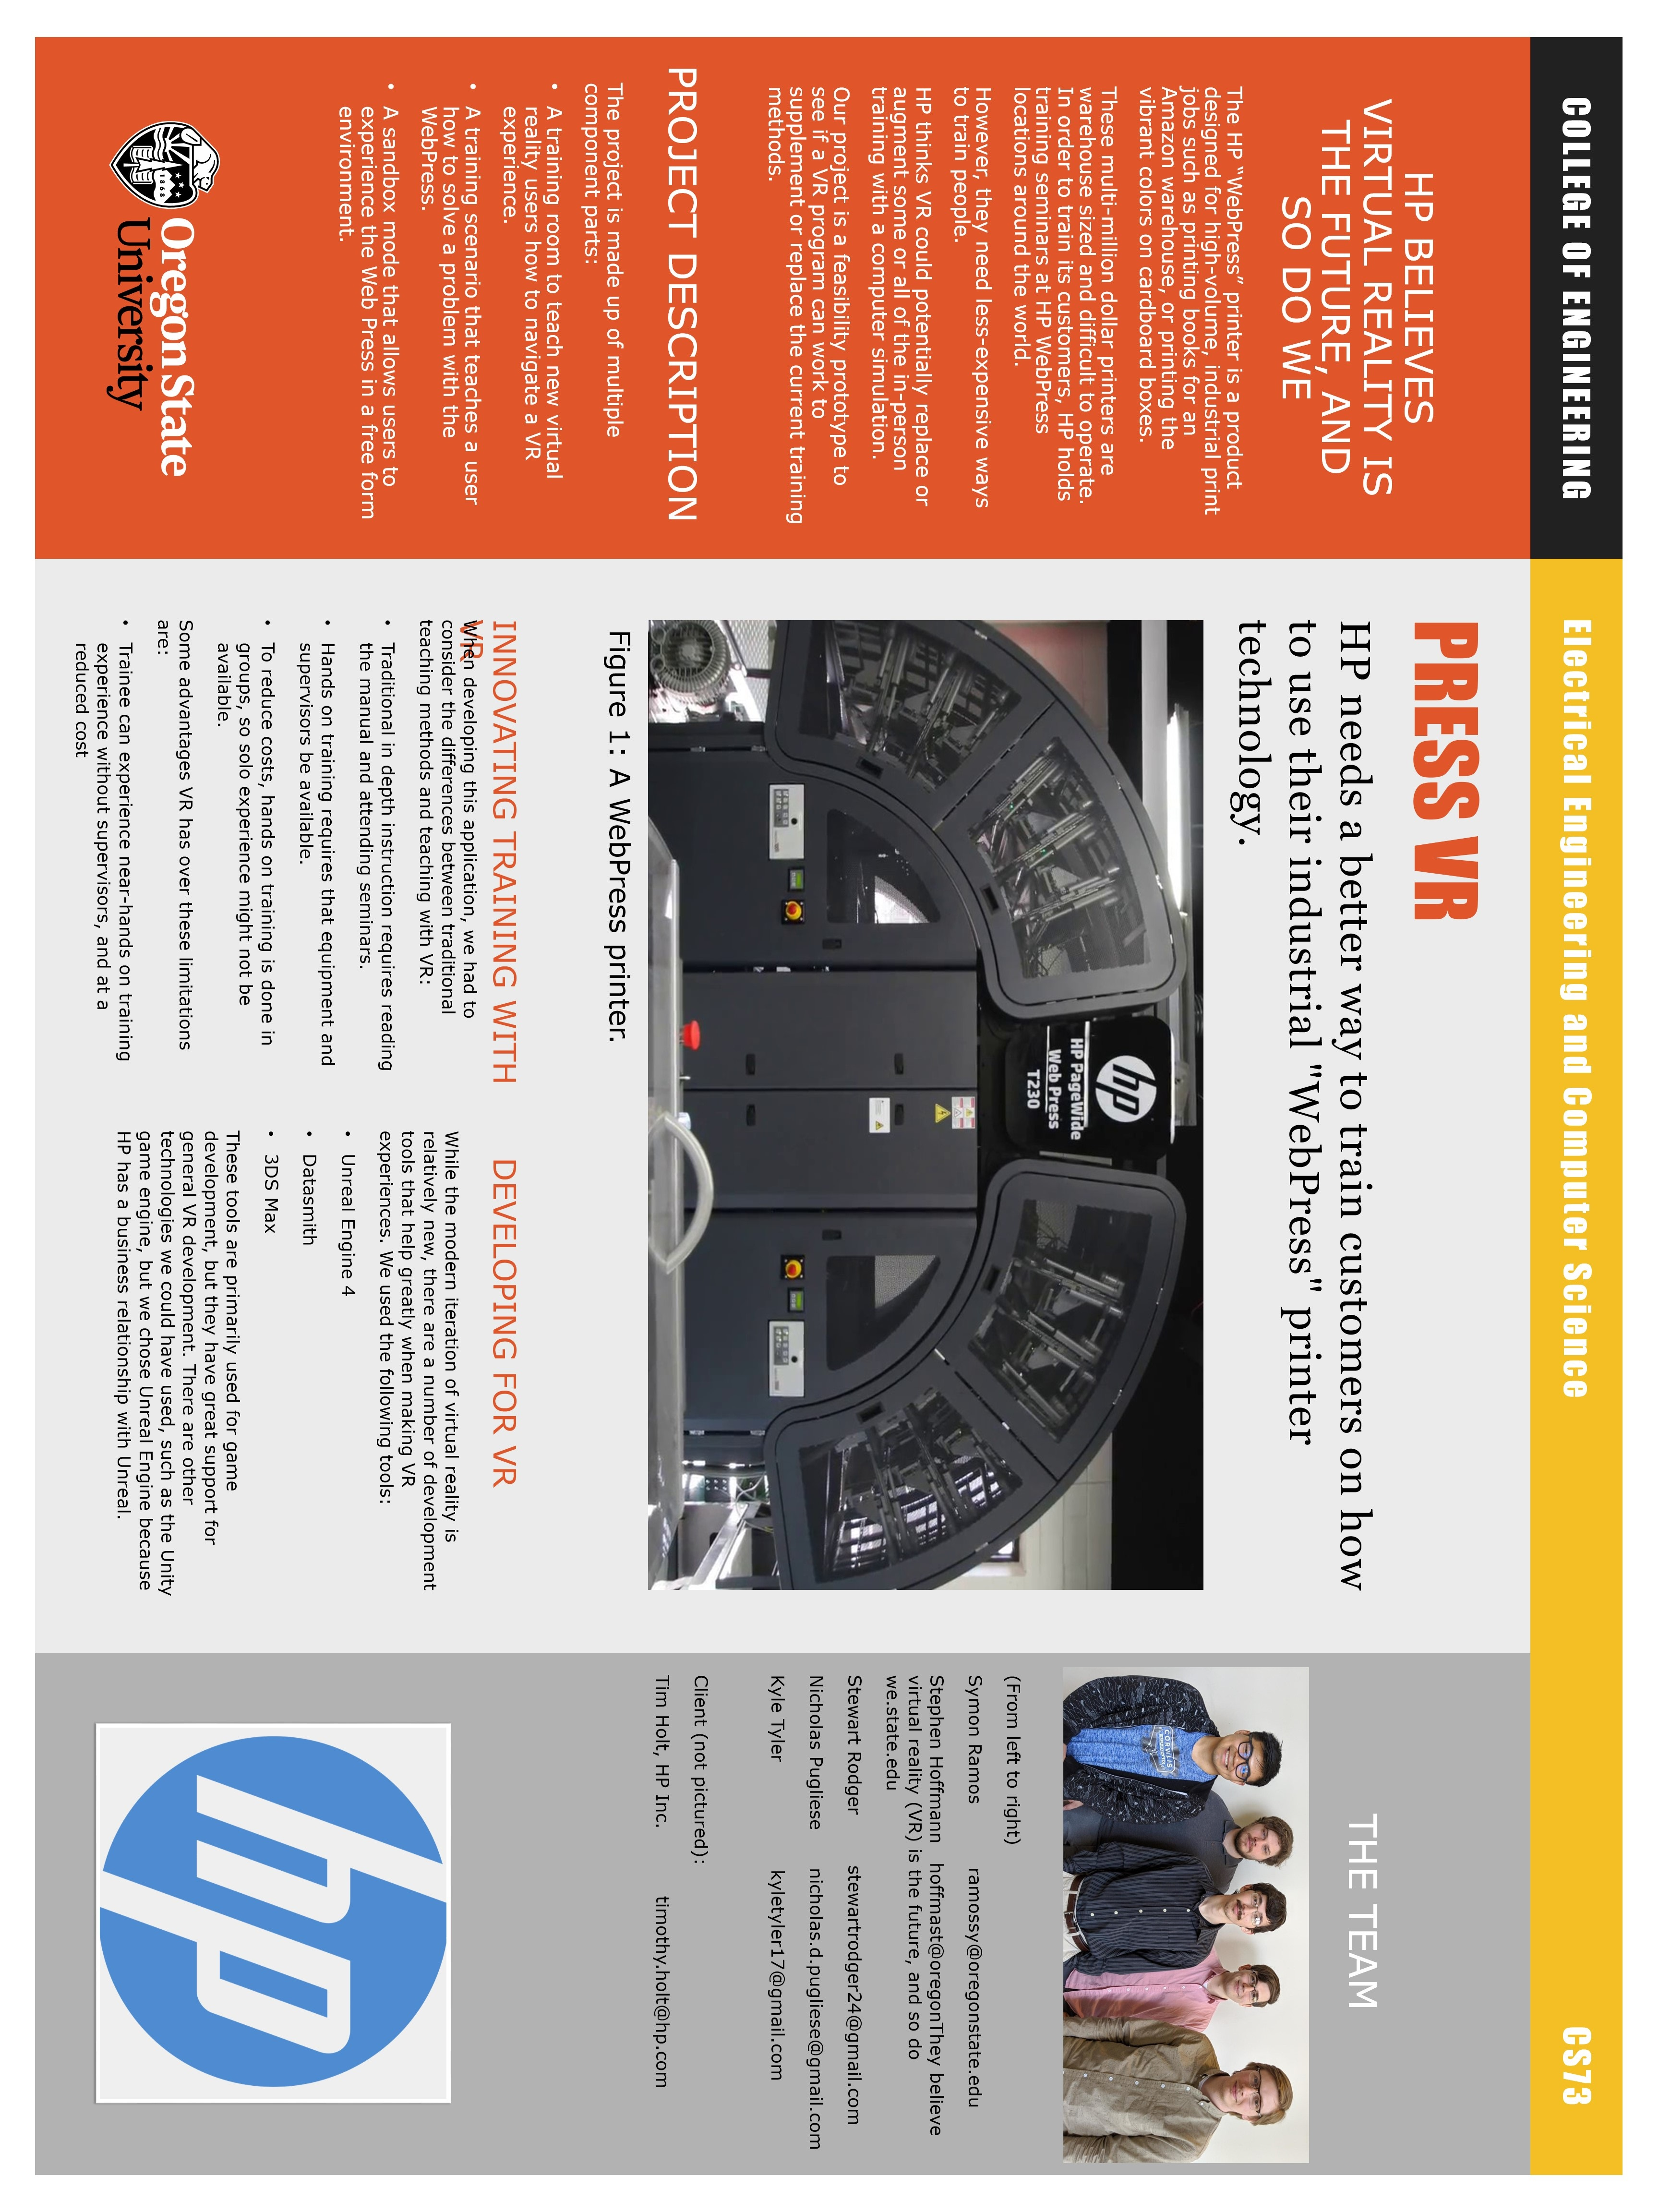
\includegraphics[scale=0.19]{poster.jpg}
    }
    \caption{Our Team's Poster}
\end{figure}

\newpage

\section{Project Documentation}
%    How does your project work? (Could include the following...) 
%        What is its structure?
%        What is its Theory of Operation?
%        Block and flow diagrams are good here.
%    How does one install your software, if any?
%    How does one run it?
%    Are there any special hardware, OS, or runtime requirements to run your software?
%    Any user guides, API documentation, etc.

\subsection{Required Software and Hardware}

The following hardware items are required to successfully run the application:

\begin{itemize}
    \item A Laptop with the following:
        \begin{itemize}
            \item Windows 10 Operating System or later
            \item Intel® Core™ i5 or better
            \item AMD Ryzen 5 1400 3.4Ghz quad core or better
            \item At least 8GB of RAM
            \item At least 10 GB of Disk Space.
            \item Bluetooth 4.0 Support 
        \end{itemize}
    \item Any of the following graphics cards: 
        \begin{itemize}
            \item Integrated Intel HD Graphics 620 or greater 
            \item DX12-capable integrated GPU
            \item Nvidia MX150 discrete GPU
            \item Nvidia GeForce GTX 1050 discrete GPU
            \item Nvidia 965M discrete GPU
            \item AMD Radeon RX 460/560
        \end{itemize}
    \item A Windows Mixed Reality Headset
    \item A Pair of Windows Mixed Reality Controllers
    \item A Bluetooth Dongle
\end{itemize}


In addition, the following software applications are also required: 
\begin{itemize}
    \item Steam 
        \begin{itemize}
            \item Steam VR Windows Headset Extension
        \end{itemize}
    \item Unreal Engine %FIXME: Put Unreal Version
    \item Windows Mixed Reality Drivers (which will be installed upon first-time use of the headset)
\end{itemize}

\subsection{Installation Guide}
\subsubsection{Download the Project}

Our project can be found on GitHub with the following link:

\noindent
\href{https://github.com/SilverGekko/cs461}{https://github.com/SilverGekko/cs461}\\

\noindent
The Executable file can be found under the "releases" section of the github page.

%\noindent In order to download the project to your local computer, please use the GitHub interface or run the following command on your terminal: 
\\
%git clone https://github.com/SilverGekko/cs461.git

In order to test the application, download the zip file from the releases page: Releases->CodeFreeze, unzip it, and run the executable file called "PressVR" contained within the subfoler "WindowsNoEditor."

\subsubsection{Configure the Windows Mixed Reality Headset}

Please refer to the link to the official setup guide below in order to successfully configure the Windows Mixed Reality Headset.

\noindent
\href{https://support.microsoft.com/en-us/help/4043101/windows-10-set-up-windows-mixed-reality}{https://support.microsoft.com/en-us/help/4043101/windows-10-set-up-windows-mixed-reality}\\

Here are additional resources to assist in the installation of the Windows Mixed Reality environment onto your computer. 

\noindent
\href{https://www.windowscentral.com/how-set-your-windows-mixed-reality-headset}{https://www.windowscentral.com/how-set-your-windows-mixed-reality-headset}\\
\noindent
\href{https://help.irisvr.com/hc/en-us/articles/115015806747-First-Time-Setup-with-Windows-Mixed-Reality-MR-Headsets}{https://help.irisvr.com/hc/en-us/articles/115015806747-First-Time-Setup-with-Windows-Mixed-Reality-MR-Headsets}\\

\subsubsection{Ensure Steam VR is used}

First, make sure Steam is installed on the current system:

\noindent
\href{https://store.steampowered.com/about/}{https://store.steampowered.com/about/}

\noindent
The Steam VR Plugin can be found here: 

\noindent 
\href{https://store.steampowered.com/app/719950/Windows_Mixed_Reality_for_SteamVR/}{https://store.steampowered.com/app/719950/Windows\_Mixed\_Reality\_for\_SteamVR/}\\

\begin{figure}[ht!]
    \centering
    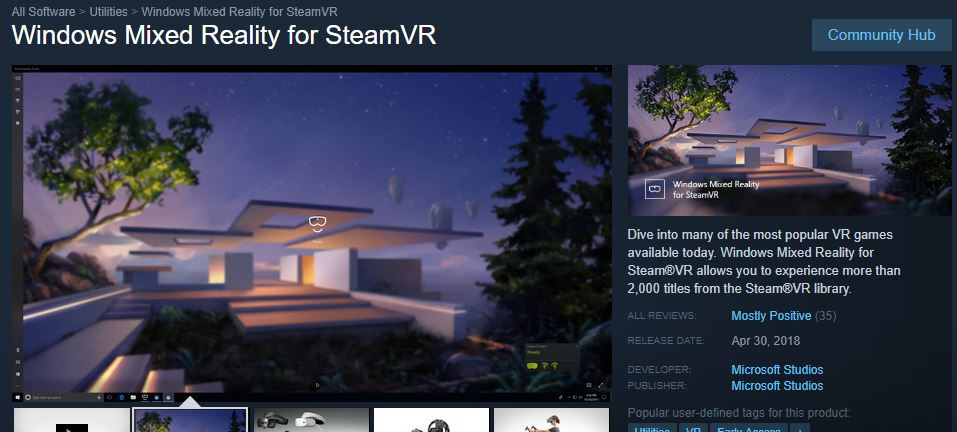
\includegraphics[width=0.85\textwidth]{steamplugin.JPG}
    \caption{Steam VR Plugin}
    \label{fig:printerModel}
\end{figure}

\subsubsection{Launch Project}

After performing the steps above, please perform the following in order to successfully launch the project: 
\begin{itemize}
    \item Find the executable file within the release zip file: PressVR->WindowsNoEditor->PressVR.exe
\end{itemize}

Once the game has launched put on the headset, pick up the controllers, and refer to section 6 for a description of the scenario.


\subsection{Basic Controls}
 Figure \ref{fig:controllers} is a description of the project's controller scheme.

\begin{figure}[ht!]
    \centering
    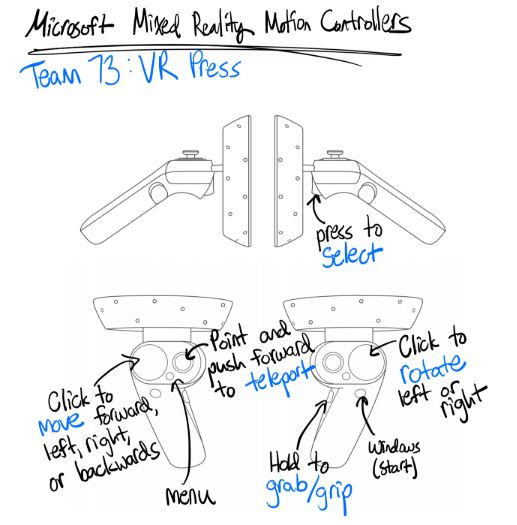
\includegraphics[width=0.85\textwidth]{VRPressInfographic.JPG}
    \caption{Windows Mixed Reality Controller Scheme}
    \label{fig:controllers}
\end{figure}


\subsubsection{Environment}

\begin{figure}[ht!]
    \centering
    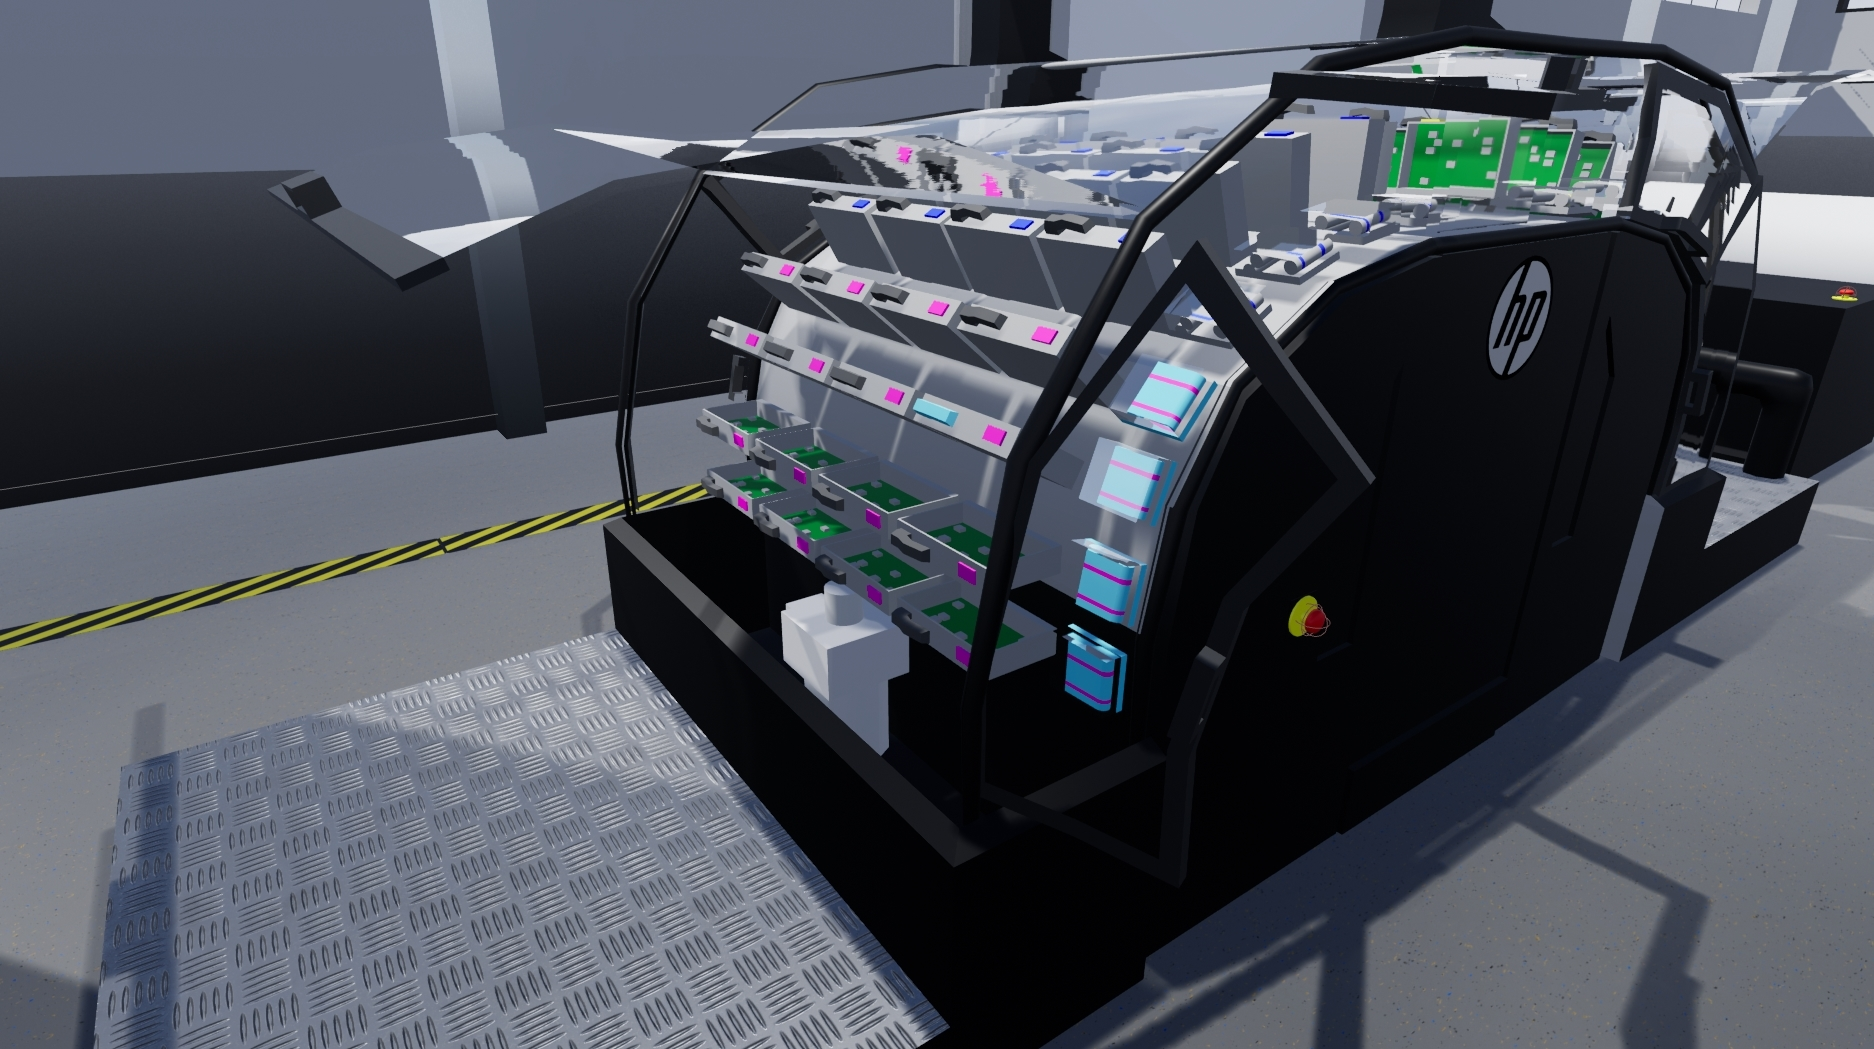
\includegraphics[width=0.85\textwidth]{press1.png}
    \caption{Web Press Printer 3D Model}
    \label{fig:printerModel}
\end{figure}

The entire virtual environment is a 3D model of a warehouse. Models we have added include the Web Press printer itself (modeled after the T240 model), ink barrels, computers, desks, chairs, an office space to serve as our tutorial room, lights, E-Stop buttons, spare printheads, tables, cabinets, and cautionary tape. The Web Press printer is comprised of multiple models, including the printer itself, the winder and unwinder (which is where the paper is fed in and out respectively), and individual printheads of different colors. 

We have also implemented basic functionality with the buttons on the Web Press and the ability to toggle lights on the printer. This is indicated in the figure below: 

\begin{figure}[ht!]
    \centering
    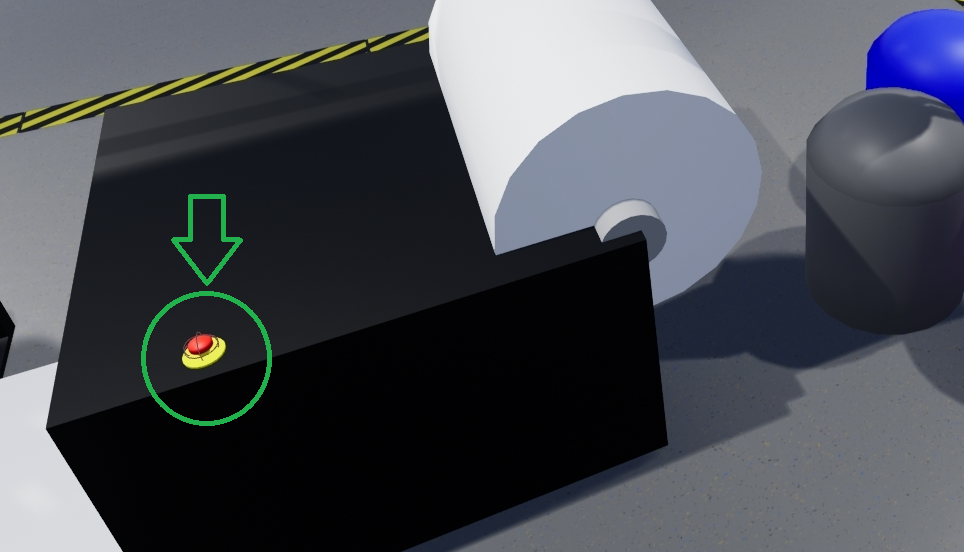
\includegraphics[width=0.85\textwidth]{button.png}
    \caption{The Emergency Stop Button}
    \label{fig:stopbutton}
\end{figure}

\subsection{Tutorial Scenario}

We have implemented a tutorial mode (created in the office space of our environment) in which the user will be tasked with performing basic actions in a cohesive narrative. 

\begin{figure}[ht!]
    \centering
    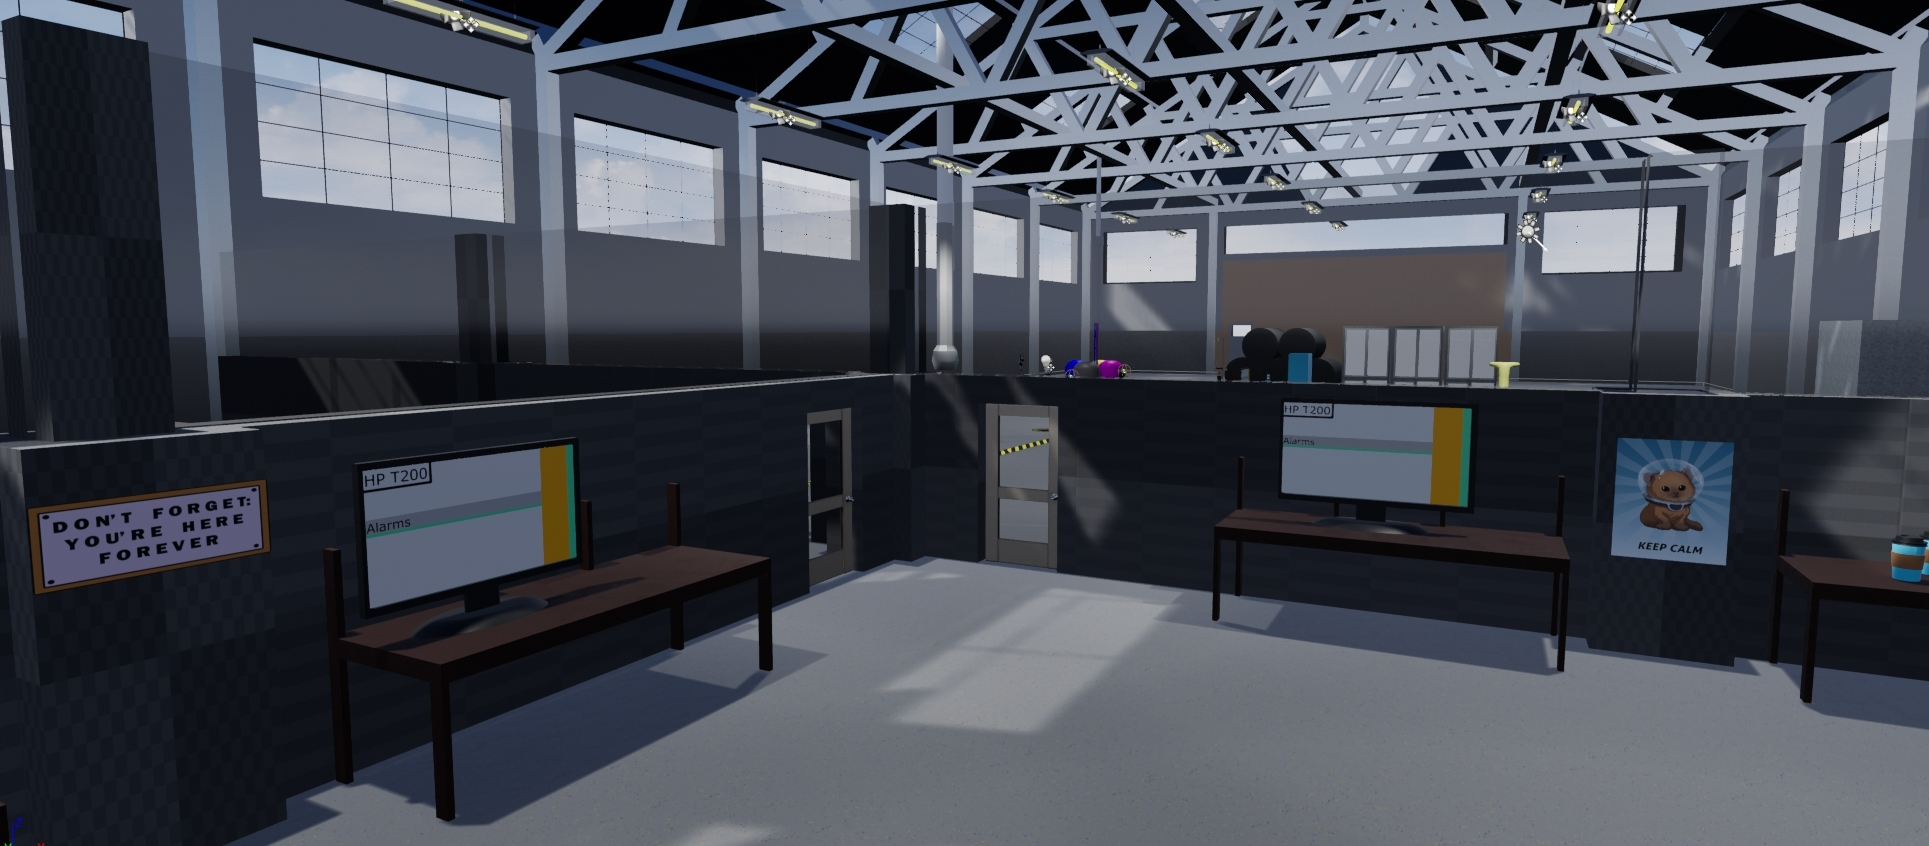
\includegraphics[width=0.85\textwidth]{tutorialSpace.png}
    \caption{The Tutorial Environment}
    \label{fig:tutorial}
\end{figure}


In this tutorial space, the user are asked to look around, focus their screen towards something, move around, grab items, and interact with the environment. 
All users are given the option of going through the tutorial mode before attempting the training module.

There are three main tutorial sections to illustrate the basic skills needed to use the Virtual Reality program:

\begin{itemize}
    \item Looking around the room in VR ("Seeing" tutorial)
    \item Using the hand-held controllers to teleport ("Moving" tutorial)
    \item Picking up objects and pressing buttons ("Interacting" tutorial)
\end{itemize}

Each of these tutorials takes places in a section of the environment designed to look like an office cubicle. This tutorial space takes place in a separate level than the Web Press itself. The user may leave this tutorial level and go to the main Web Press level by clicking a button on the user interface. The tutorial instructs the user to do this once the three tutorials listed above are done, but an experienced user may exit the tutorial at any time by accessing the same menu.

\subsubsubsection{Sight}
The seeing tutorial teaches the user that they may look around with full 3D motion while wearing the headset. The tutorial is completed by making the user point to an onscreen crosshair at a computer monitor on a desk. This process is repeated on three total monitors ranging from in front of the user, to almost directly behind them. The idea is to force the user to physically turn their body around so they learn the extent of the control they have over the viewport with the headset.

\subsubsubsection{Movement}
The moving tutorial teaches the user that they can move around the virtual space by pressing a button on the controller, pointing, and releasing to teleport to that location. The tutorial is completed when the user teleports away from the starting position. This teaches the user how to move around the environment, which they will need to do to complete the training scenarios.   

\subsubsubsection{Interaction}
The interacting tutorial teaches the user that there are objects in the virtual environment that may be interacted with using the handheld controllers by moving the controller over the object in the virtual space and holding down the trigger button. All of the objects in the virtual space that may be grabbed like this are colored the same sky blue color as shown in figure \ref{fig:skyblue}.

\begin{figure}[ht!]
    \centering
    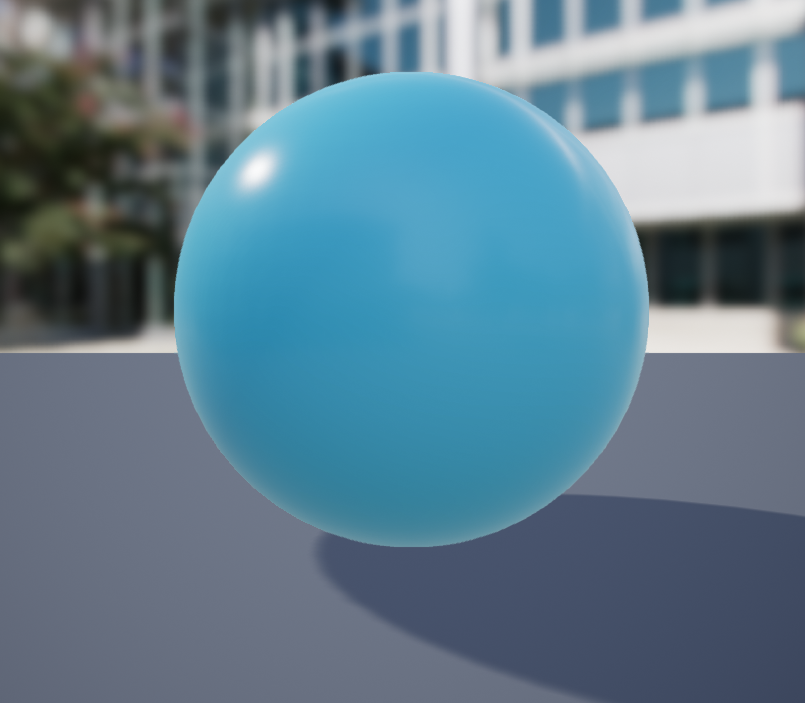
\includegraphics[scale=0.5]{touchMeBlue.png}
    \caption{The specific shade of blue that informs the user they may pick up and manipulate the object.}
    \label{fig:skyblue}
\end{figure}

\subsection{Training Scenario}

\subsubsection{Replacing Printheads}

The T2XX Web Press Operating Manual outlines a sequential series of steps that the user has to complete in order to successfully remove the existing printhead and insert the new one. In a later section detailing common troubleshooting scenarios, several scenarios where the replacement of printheads would be applicable are included, such as when a printhead is overheating. Figure 8 below outlines the user workflow of the replacement of printheads. It should be followed until the voice over informs the user that the scenario is complete. If at any point the user gets stuck they may open the menu (see figure 3) and select the training scenario again to restart the scenario.

\begin{figure}[ht!]
    \centering
    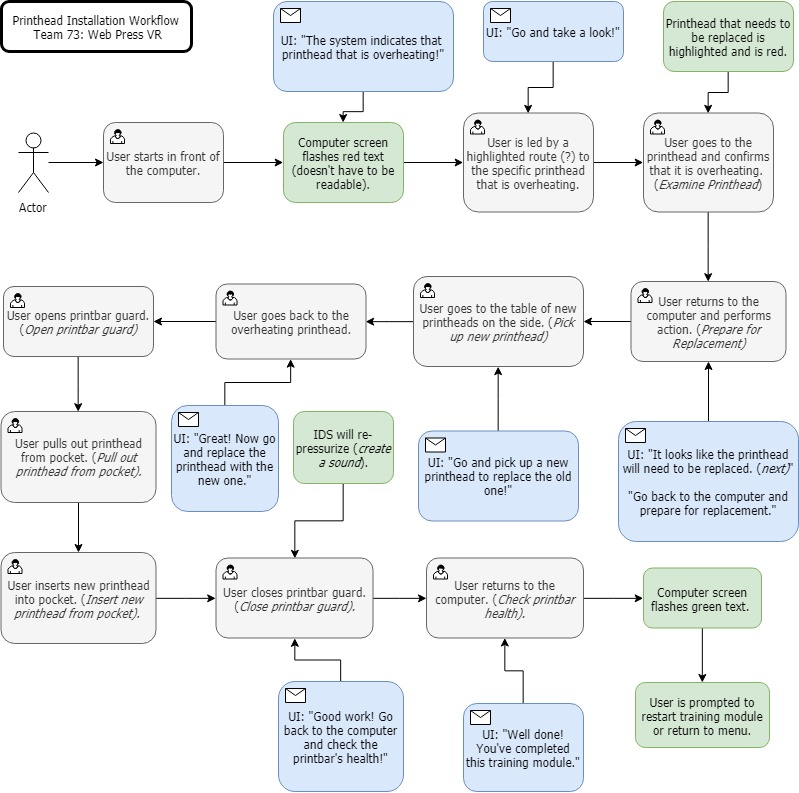
\includegraphics[width=0.85\textwidth]{PrintheadInstallationWorkflow.jpg}
    \caption{The Printhead Installation Workflow}
    \label{fig:workflow}
\end{figure}
\subsection{Developer Notes}

Please contact HP personnel for more information and inquiries should further development be desired.

Future Implementation that could be considered is as follows: 
\begin{itemize}
    \item Additional training scenarios, such as the replacement of printer wiper cassettes.
    \item Refinement of 3D environment.
    \item Support for additional headsets.
    \item Additional Web Press Models. 
    \item An expanded warehouse environment that includes office space.
\end{itemize}

\subsection{Version Log}
This section was last updated on 6/5/19.





\newpage
\section{Recommended Technical Resources for Learning More}

%    What web sites were helpful? (Listed in order of helpfulness.)
%    What, if any, reference books really helped?
%    Were there any people on campus that were really helpful?

Websites:

\begin{itemize}
    \item Unreal Engine Documentation:
    \\https://docs.unrealengine.com/en-US/Platforms/MR/WMRSDKRequirements/index.html
    \item Youtube (an example tutorial):
    \\https://www.youtube.com/watch?v=j8gjvKyaQuU
    \item Unreal Engine AnswerHub:
    \\https://answers.unrealengine.com/index.html
    \item Unreal Engine Forums:
    \\https://forums.unrealengine.com/
    \item Unreal Engine Reddit:
    \\https://www.reddit.com/r/unrealengine/
    \\item Oculus Documentation:
    \\https://developer.oculus.com/documentation
\end{itemize}

People:

\begin{itemize}
    \item Professor de Amicis was a great resource and taught those of us in his CS419 (VR and AR development) class a lot about virtual reality and developing with Unreal Engine.
\end{itemize}

\section{Conclusions and Reflections}

\subsection{Nicholas Pugliese}
\begin{enumerate}
    \item \textbf{What technical information did you learn?}
    
    I learned a lot about how Games/Graphics projects are developed using more advanced software like Unreal Engine. There is a lot more story-boarding that goes on rather than code writing. The biggest technical thing I had to learn this term was how to develop for Virtual Reality. Since VR technology is so new it's really under-documented, which makes debugging hard. I also learned that developing in a physics engine can lead to very weird bugs when working with turning physics on and off. We have a bug in the final build where if you place an object in a trash can, both the object and the trash can will fly off into oblivion. I also learned how to build a 3D game project in the Unreal Engine, import resources from Sketchup and CAD files, place them in a scene, render the scene, and export it to an executable for demontration on another machine.
    
    \item \textbf{What non-technical information did you learn?}
    
    I learned a lot about the bureaucracy about getting a new, innovative idea off the ground in a company that doesn't want to spend money. This "using VR to teach" idea is very new within HP, and people are exicted about. However, most people currently see it as something they want to get into, but do not wish to spend the resources on a prototype that might never amount to what they needed it to be.
    
    \item \textbf{What have you learned about project work?}
    
    I learned that no matter what, tasks in the project will take longer to complete than you think they will. The best laid plans of mice and men often go awry, as they say. I also learned that working with team member pair programming can lead to either the best code I've ever written, or close to it.
    
    \item \textbf{What have you learned about project management?}
    
    This project was the first that I've participated in where we used software tools to help tract what needed to be done. I think it helped us a ton with realizing what needed to be done overall instead of getting lost in the weeds with certain details that might not matter until later, and focus on getting the core project done. I learned that spending time organizing is equally if not more important than doing the actual work. If you don't know what you need to do, you can't do it.
    
    \item \textbf{What have you learned about working in teams?}
    
    Much like parallel programming, you lose performance when working in a group due to inter-process communication. All group members have to spend time talking about what they did so the others don't re-do work or accidentally break things. The most important part is to have patience and to trust what your group is doing. I tend to worry too much about everything, so I had to learn to take a step back and let my team do their parts while I did mine.
    
    \item \textbf{If you could do it all over, what would you do differently?}
    
    I would have broken down everything we possibly could into sub-tasks and given those tasks due dates. We kinda did break everything up, but we left them as needed to be completed whenever someone finished it. I think we could have polished the features we have, as well as created a wider variety of training modes and scenarios. This is mostly hindsight, since it took the time in the first place because we were learning everything as we went.
    
\end{enumerate}
\subsection{Kyle Tyler}
\begin{enumerate}
    \item \textbf{What technical information did you learn?}
    
    I learned a lot about game engine technology and game development in general. Unreal Engine was a tool I had never used before, so learning to make things work with it was a real technical challenge, but it definitely made me a stronger developer. Another thing I learned was about the current state of virtual reality hardware and software production. It is a young and growing field, so there was a lot of information that was hard to find or cutting edge, which was pretty exciting. 
    
    \item \textbf{What non-technical information did you learn?}
    
    I learned a lot about the VR landscape and some of the work that is being done in that field. I talked to VR professionals who do this for a living, and learned how the field has grown with the advent of cheaper technology and improved hardware. 
    
    \item \textbf{What have you learned about project work?}
    
    I learned that the only important thing with project work is the project itself. It can be easy to get distracted and work on tiny pieces because they are fun and interesting, but that will hurt the project in the long run. The critical pieces need to be implemented as soon as possible, and everything else will be built up around that. 
    
    \item \textbf{What have you learned about project management?}
    
    In terms of project management I learned a lot about how important plans are, but also being flexible and moving goals. There were many times where we had to reduce scope and move priorities around.
    
    \item \textbf{What have you learned about working in teams?}
    
    I learned about the importance of communication, having a plan, and knowing what everybody is working on at all times. I have never worked on such a big project with so many people, so it was critical to quickly learn that everybody needs to be on the same page at all times. If it feels like you are communicating too much, you are probably communicating just about enough.
    
    \item \textbf{If you could do it all over, what would you do differently?}
    
    I would have used a more common and well-supported VR headset, because we ran into a lot of problems trying to get our hardware too work well with software who only supported our HMD in a beta version. I also would have started working on the major pieces sooner, instead of tinkering with little fun parts first. That was hard because we were all still learning how to use the technology, so if I started again I would have a lot more knowledge that would make me much more productive.
    
\end{enumerate}
\subsection{Stephen Hoffmann}
\begin{enumerate}
    \item \textbf{What technical information did you learn?}
    
    I didn't know anything about unreal and how to create games in Unreal. I was able to learn a lot of Unreal's tool set, as well as incorporating skills I already have into unreal, such as programming and 3d modeling for VR applications.
    
    \item \textbf{What non-technical information did you learn?}
    
    Discovering VR applications and how we can incorporate VR for future applications that are such as technical training for real world scenarios. The VR workspace is much larger than just gaming, and that is important information.
    
    \item \textbf{What have you learned about project work?}
    
    Project work is something we have to do on big projects, and this project helped me learn the important of roles and good divisions of works. I think our team excelled in this, which made hitting deadlines much easier.
    
    \item \textbf{What have you learned about project management?}
    
    Project management came down to knowing deadlines and the feasible amount of work each team member can do. We where always outlining future work, and estimations on how long tasks would  take. This helped manage our time and help achieve our goals.
    
    \item \textbf{What have you learned about working in teams?}
    
    Everyone has different preferences on how they work best, with also what kinds of tasks they like the best. We where good at utilizing each others personal strengths and that helped us trust and rely on each other that we would get work done.
    
    \item \textbf{If you could do it all over, what would you do differently?}
    
    Start development in the first term, even if we weren't suppose to. Starting to build a basic work environment to play with could have allowed each of us to learn faster, which could have lead to more outreaching goals for our program, such as another training scenario.
    
\end{enumerate}
\subsection{Symon Ramos}
\begin{enumerate}
    \item \textbf{What technical information did you learn?}
    \\
    I learned basic development with the Unreal interface. One of the things I was tasked with was helping to create the inside environment of the warehouse where the scenario took place. We used Sketch-Up in tandem with Unreal in order to add 3D models into the virtual space. I also learned troubleshooting skills and concepts relevant to Virtual Reality development, such as the need of using certain software (EX: SteamVR) in order to boot systems rather than relying solely on the software that came with the hardware. 
    \\\\
    I also learned that there is a lot of substantial value in creating Virtual Reality systems that aren't necessarily high-fidelity, but are capable of getting the point across. We decided to create the environment in a low-poly state that enabled us to efficiently and effectively convey the various steps that we wanted the operator to be able to undergo. This was all in attempts to promote and facilitate learning amongst our participants. 
        
    \item \textbf{What non-technical information did you learn?}
    
    I learned a great deal about the many tasks a Web Press operator has to undertake in order to monitor and repair a Web Press printer. We had the pleasure of being able to visit the HP site and tour their facility, as well as the Web Press printers we would soon model. I was also mainly tasked with the research and analysis of the various aspects of the Web Press printer through the manuals that our client provided for us. I was able to become well-versed in the many applications to which a Web Press would need maintenance and supervision, such as when a printhead is overheating or when a wiper is in need of replacement. 
    
    \item \textbf{What have you learned about project work?}
    
    I found in this project that there are many different roles that can be fulfilled, all of which are necessary in order to create and bring forth a good project. I believe that this is something that I can very easily foresee being prevalent in industry: the delegation of tasks and roles to different team members so that their expertise can fit according to their ability while at the same time allowing leeway for all team members to learn from each other and gain experience in all levels and facets of a given project.
    
    \item \textbf{What have you learned about project management?}
    
    Project management, as I discovered in this project, is hugely necessary in the development and structure of the project. Without good project management, while a task might end up getting completed, could have overburdened the entire team with a negative experience and an unwarranted disorganization that is only alleviated with successful project management. 
    \\
    I also learned that project management pertains to the entire team and not just a particular individual. While we were fortunate enough to be able to have a team member serve as the de facto project manager, we managed our own respective roles and the roles of others to the degree that it enabled us to keep each other accountable throughout the entire process, thereby promoting quality work.
    
    \item \textbf{What have you learned about working in teams?}
    
    When working in teams of 5 for a project of this scope, I learned that the delegation of tasks and the adoption of roles is integral to the effectiveness of the project's implementation and can also greatly improve the quality of the final result due to the honed-in focus of the tasks given to us. Another advantage to working in a team of this size and caliber were the many opportunities to pair program and work on a particular task or troubleshoot a particular issue with. Having different backgrounds and levels of expertise enabled us to share knowledge with other team members and grow our entire knowledge base in this way.
    
    \item \textbf{If you could do it all over, what would you do differently?}
    
    While I enjoyed the project throughout its entire duration, I would, in retrospect, be more proactive about gaining feedback from our client and making sure, on a week-to-week basis, gathering his thoughts on our current vision. While it worked for this project, I feel like it would be a good habit to develop for industry to have a very close and interactive relationship with management. I would also most likely seek out other facets of the project with greater intensity to become even more familiar with Virtual Reality design and implementation.
    
\end{enumerate}
\subsection{Stewart Rodger}
\begin{enumerate}
    \item \textbf{What technical information did you learn?}
    
    I already had basic familiarity with the Unreal Engine, however over the course of this project I learned the ins and outs of program flow within an Unreal Blueprint, Sound implementation, UI/Mentu implementation, and general programming experience within the same engine. I also learned about interfacing custom programs in unreal with both Microsoft Mixed Reality Headsets and the Oculus Rift.
    
    \item \textbf{What non-technical information did you learn?}
    
    On the non-technical side I learned a lot about how users can respond to a specific interface or task flow that may seem obvious to every member of the team, but may fly over the head of a new user. 
    
    \item \textbf{What have you learned about project work?}
    
    This project has fully convinced me of the importance of early documentation and implementation research in project work. To make sure the project goes as well as possible it is important to have the project appropriately defined, with specific goals, tools, and timelines. 
    
    \item \textbf{What have you learned about project management?}
    
    This project has reinforced my understanding of project management, specifically that the project should be broken down into tasks early, and the tasks should be issued to specific team members or selected by them as soon as possible to maintain productiveness.
    
    \item \textbf{What have you learned about working in teams?}
    
    From this project I learned that teamwork will often not be "equal", and that it is more important to play to all members strengths to get the best version of the result out.
    
    \item \textbf{If you could do it all over, what would you do differently?}
    
    If I could do it all over again I would condense the first term into 1 month, and try and get access to the hardware much earlier than we were able to. We often found ourselves going over repeated information for the assignments and would have befitted from being able to begin work sooner.
    
\end{enumerate}

\end{document}
